\documentclass{article}
\usepackage[utf8]{inputenc}
\usepackage[T1]{fontenc}
\usepackage{amssymb}
\usepackage{natbib}
\usepackage{graphicx}
\usepackage{mathtools}
\usepackage{amsthm}
\usepackage{tikz}
\usepackage{caption}
\usepackage{mathrsfs}
\usepackage{hyperref} 
\usepackage{csquotes}
\usetikzlibrary{arrows}
\usepackage[labelformat=empty]{subfig}
\usepackage[noend]{algpseudocode}
\usepackage{algorithm}
\usepackage{listings}
\usepackage{enumitem}
\usepackage[a4paper,top=4cm,bottom=3cm,left=3.5cm,right=3.5cm]{geometry} % margens
\usepackage{pgf,pgfplots}
\pgfplotsset{compat=1.15}
\usepackage{mathrsfs}
\usetikzlibrary{arrows}
\renewcommand{\algorithmicrequire}{\textbf{Input:}}
\renewcommand{\algorithmicensure}{\textbf{Output:}}
\renewcommand{\And}{\textbf{and} }
\newcommand{\Or}{\textbf{or} }
\newcommand{\tdots}{\,.\,.\,} % in place of \ldots

\DeclarePairedDelimiter\ceil{\lceil}{\rceil}
\DeclarePairedDelimiter\floor{\lfloor}{\rfloor}

\def\realnumbers{\mathbb{R}}
\def\bigo{\mathcal{O}}
\newtheorem{theorem}{Theorem}
\newtheorem{definition}{Definition}
\newtheorem{proposition}{Proposition}
\newtheorem{lemma}{Lemma}
\newtheorem{problem}{Problem}
\newtheorem{corollary}{Corollary}

\fontsize{60}{62}\usefont{OT1}{cmr}{m}{n}{\selectfont}
\usepackage{fancyhdr}
\pagestyle{fancy}
\fancyhf{}

\newcommand{\chaptermark}[1]{\markboth{\MakeUppercase{#1}}{}}
\renewcommand{\sectionmark}[1]{\markright{\MakeUppercase{#1}}{}}
\renewcommand{\subsectionmark}[1]{}
\renewcommand{\headrulewidth}{0pt}
\fancyhead[R]{{\footnotesize\rightmark}}
\fancyhead[L]{{\footnotesize\leftmark}}
\fancyfoot[C]{{\thepage}}
%\setcounter{tocdepth}{2}
\setlength{\headheight}{13.6pt} 

\newcommand{\RR}{\realnumbers}

\begin{document}

\title{Algorithms for the 2D Ham Sandwich Problem}
\author{Giovanna Kobus Conrado}
\date{\today}
\maketitle

% \begin{document}

\begin{abstract}
Given two disjoint sets $P_1$ and $P_2$ in $\realnumbers^2 $, a two-dimensional \textit{ham sandwich cut} is a line that bisects both $P_1$ and $P_2$ simultaneously. The \textit{ham sandwich problem} consists of finding such a line. A linear-time algorithm to solve this problem was proposed by Chi-Yuan Lo, Ji\v{r}í Matou\v{s}ek and William Steiger~\cite{LoMS1994}. We expand on their paper, detailing the steps needed to implement the algorithm, presenting both  pseudo-code and a C++ implementation for it and providing some of the knowledge needed to understand both the algorithm and why it works.
\end{abstract}

\newpage
\section{Introduction}

\begin{definition}
\label{bisect_definition}
A line $\ell$ is said to bisect the set $P$ of points in $\realnumbers^2$ if no more than $\frac{|P|}{2}$ points of~$P$ lie on either of the open half-planes defined by $\ell$.
\end{definition}

\begin{figure}[!ht]%
    \centering
    \subfloat[]{
        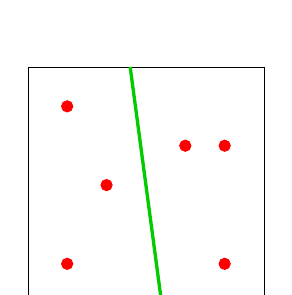
\begin{tikzpicture}
        
        \draw[black, ultra thin] (0,0) rectangle (3,3);
        
        \draw [green!80!black, very thick] (1.7,0) -- (1.3,3);
        
        \filldraw [red] (0.5,0.5) circle (2pt);
        \filldraw [red] (1,1.5) circle (2pt);
        \filldraw [red] (2.5,2) circle (2pt);
        \filldraw [red] (2,2) circle (2pt);
        \filldraw [red] (0.5,2.5) circle (2pt);
        \filldraw [red] (2.5,0.5) circle (2pt);
        
        \end{tikzpicture}
    }
    \qquad
    \subfloat[]{
       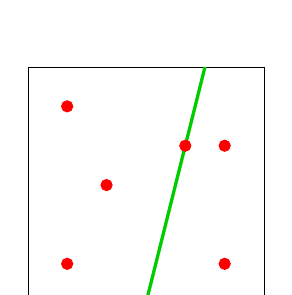
\begin{tikzpicture}
        
        \draw[black, ultra thin] (0,0) rectangle (3,3);
        
        \draw [green!80!black, very thick] (1.5,0) -- (2.25,3);
        
        \filldraw [red] (0.5,0.5) circle (2pt);
        \filldraw [red] (1,1.5) circle (2pt);
        \filldraw [red] (2.5,2) circle (2pt);
        \filldraw [red] (2,2) circle (2pt);
        \filldraw [red] (0.5,2.5) circle (2pt);
        \filldraw [red] (2.5,0.5) circle (2pt);
        
        \end{tikzpicture}
    }%
    \qquad
    \subfloat[]{
        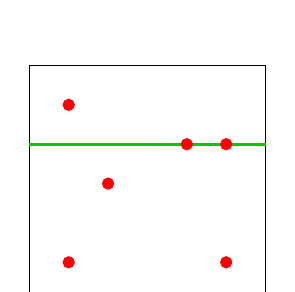
\begin{tikzpicture}
        
        \draw[black, ultra thin] (0,0) rectangle (3,3);
        
        \draw [green!80!black, very thick] (0,2) -- (3,2);
        
        \filldraw [red] (0.5,0.5) circle (2pt);
        \filldraw [red] (1,1.5) circle (2pt);
        \filldraw [red] (2.5,2) circle (2pt);
        \filldraw [red] (2,2) circle (2pt);
        \filldraw [red] (0.5,2.5) circle (2pt);
        \filldraw [red] (2.5,0.5) circle (2pt);
        
        \end{tikzpicture}
    }%
    \caption{In all the images above, the line bisects the set of points.}%
    \label{bisect_examples_figure}%
\end{figure}

Let the pair $(x,y)$ represent the a point and the pair $(m,b)$ represent the line $y=m\cdot x+b$.  
Note that vertical lines do not have such representation. 
From now on, the term \emph{line} refers always to non-vertical lines. 

We can easily check if such a line bisects a set of points in linear time using Algorithm~\ref{bisects}.

\newcommand{\true}{\textsc{true}}
\newcommand{\false}{\textsc{false}}

\begin{algorithm}
\begin{algorithmic}[1]
\Require{a line $\ell$ and a set $P$ of points}
\Ensure{\true\ if $\ell$ bisects $P$ and \false\ otherwise}

\State $below \gets 0$
\State $above \gets 0$
\For{each point $p$ in $P$}
    \If{$p.y < \ell.m \cdot p.x + \ell.b$} $below \gets below + 1$
    \EndIf
    \If{$p.y > \ell.m \cdot p.x + \ell.b$} $above \gets above + 1$
    \EndIf
\EndFor
\State \Return $below \leq \frac{|P|}{2}$ \And $above \leq \frac{|P|}{2}$
\end{algorithmic}
\caption{\textsc{Bisects}($\ell$, $P$)}
\label{bisects}
\end{algorithm}

\begin{definition}\label{ham_sandwich_cut_definition}
A ham sandwich cut of two sets $P_1$ and $P_2$ of points in $\realnumbers^2 $ is a line that bisects both $P_1$ and $P_2$ simultaneously.
\end{definition}

\begin{problem}[Two-Dimensional Discrete Ham Sandwich Problem]\label{ham_sandwich_problem}
Given two sets $P_1$ and~$P_2$ of points in $\RR^2$, find a ham sandwich cut for $P_1$ and $P_2$.
\end{problem}

It is not obvious, but such a cut always exists.  
In Section~\ref{sec:existence}, we will show a constructive proof for when the sets $P_1$ and $P_2$ are in general position. 
We would like to find a ham sandwich cut as efficiently as possible. 
% In what follows, we denote by $n$ the number $|P_1|+|P_2|$.

\begin{figure}[!htbp]%
    \centering
    \subfloat[]{
        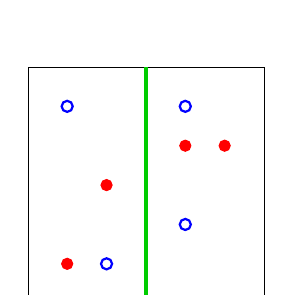
\begin{tikzpicture}
        
        \draw[black, ultra thin] (0,0) rectangle (3,3);
        
        \draw [green!80!black, very thick] (1.5,0) -- (1.5,3);
        
        \filldraw [red] (0.5,0.5) circle (2pt);
        \filldraw [red] (1,1.5) circle (2pt);
        \filldraw [red] (2.5,2) circle (2pt);
        \filldraw [red] (2,2) circle (2pt);
        
        \draw [blue,thick] (1,0.5) circle (2pt);
        \draw [blue,thick] (2,2.5) circle (2pt);
        \draw [blue,thick] (2,1) circle (2pt);
        \draw [blue,thick] (0.5,2.5) circle (2pt);
        
        \end{tikzpicture}
    }%
    \qquad
    \subfloat[]{
        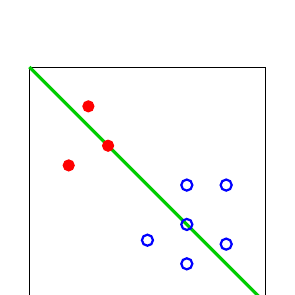
\begin{tikzpicture}
        
        \draw[black, ultra thin] (0,0) rectangle (3,3);
        
        \draw [green!80!black, very thick] (3,0) -- (0,3);
        
        \filldraw [red] (0.5,1.75) circle (2pt);
        \filldraw [red] (1,2) circle (2pt);
        \filldraw [red] (0.75,2.5) circle (2pt);
        
        \draw [blue,thick](2,0.5) circle (2pt);
        \draw [blue,thick](2,1) circle (2pt);
        \draw [blue,thick](2,1.5) circle (2pt);
        \draw [blue,thick](2.5,1.5) circle (2pt);
        \draw [blue,thick](1.5,0.8) circle (2pt);
        \draw [blue,thick](2.5,0.75) circle (2pt);
        
        \end{tikzpicture}
    }%
    \qquad
    \subfloat[]{
        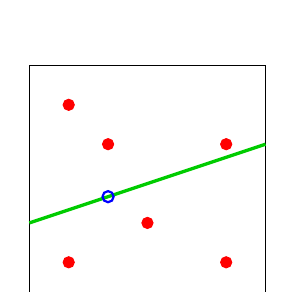
\begin{tikzpicture}
        
        \draw[black, ultra thin] (0,0) rectangle (3,3);
        
        \draw [green!80!black, very thick] (0,1) -- (3,2);
        
        \filldraw [red] (0.5,0.5) circle (2pt);
        \filldraw [red] (1,2) circle (2pt);
        \filldraw [red] (2.5,2) circle (2pt);
        \filldraw [red] (1.5,1) circle (2pt);
        \filldraw [red] (0.5,2.5) circle (2pt);
        \filldraw [red] (2.5,0.5) circle (2pt);
        
        \draw [blue,thick](1,4/3) circle (2pt);
        
        \label{ham_sandwich_cut_examples_figure}
        \end{tikzpicture}
    }%
    \caption{The points in red (filled) are in $P_1$ and the points in blue (not filled) are in $P_2$. 
             The lines are ham sandwich cuts of $P_1$ and $P_2$.}%
\end{figure}

To make the problem easier to solve, we will need some observations.

\begin{proposition}
\label{lies_on_odd_proposition}
Let $P$ be a set of points in $\realnumbers^2$ such that $|P|$ is odd and $\ell$ be a line that bisects $P$. There is a point in $P$ that lies on $\ell$.
\end{proposition}
\begin{proof}
By definition, any line that bisects $P$ must leave no more than $\frac{|P|}{2}$ points on either of its sides. Since the number of points that lie strictly on some side of $\ell$ is always an integer, that line must leave no more than $\floor{\frac{|P|}{2}} = \frac{|P|-1}{2}$ points on either of its sides. So we have a maximum of $|P|-1$ points that lie strictly on any side of $\ell$. Thus, at least one point of $P$ has to lie on $\ell$.
\end{proof}

\begin{proposition}
\label{can_solve_odd_proposition}
Let $P$ be a set of points in $\realnumbers^2$ such that $|P|$ is even. For every point $x\in P$, any line that bisects $P-\{x\}$ also bisects $P$.
\end{proposition}
\begin{proof}
Since $|P|$ is even, $|P-\{x\}|$ is odd. Let $\ell$ be a line that bisects $P-\{x\}$. From Proposition~\ref{lies_on_odd_proposition}, at least one point from $P-\{x\}$ lies on $\ell$.  Therefore, at most $\frac{|P-\{x\}|-1}{2}=\frac{|P|-2}{2}$ points lie on either side of $\ell$. So, no matter where $x$ lies, at most $\frac{|P|}{2}$ point will lie on either side of $\ell$, which, by definition, implies that $\ell$ bisects~$P$.
\end{proof}

From Proposition~\ref{can_solve_odd_proposition}, we may assume without loss of generality that both $P_1$ and~$P_2$ have an odd number of points. Otherwise, we can just remove any point from the even sets and a solution to the modified instance will also be a solution to the original instance.
Now Proposition~\ref{lies_on_odd_proposition} can give us a powerful observation: a ham sandwich cut goes through at least one point from $P_1$ and one point from $P_2$. That, and the guarantee that the cut always exists, gives us a naive $\bigo(n^3)$ algorithm to solve Problem~\ref{ham_sandwich_problem}, where $n = |P_1|+|P_2|$.

Algorithm~\ref{n3_algorithm} goes through every point in $P_1$ and every point in $P_2$ and checks if the line that passes by both of these points is a ham sandwich cut. As we are representing lines by their equations $y=mx+b$, we assume that there are no two points in $P_1$ and $P_2$ with the same x-coordinate.  In fact, to facilitate the exposition, we consider only sets of points in general position.

% arrumar
\begin{algorithm}
\begin{algorithmic}[1]
\Require{two nonempty sets $P_1$ and $P_2$ of points in general position}
\Ensure{a ham sandwich cut for $P_1$ and $P_2$}

 \For{each point $p_1$ in $P_1$}
  \For{each point $p_2$ in $P_2$}
    \State $m \gets \frac{p_2.y - p_1.y}{p_1.x - p_2.x}$
    \State $b \gets p_1.y - m \cdot p_1.x $
        \State $\ell \gets (m,b)$ \hfill {\small \textcolor{gray}{$\rhd$ line that contains $p_1$ and $p_2$}}
    \If{\textsc{Bisects}($\ell$, $P_1$) \And \textsc{Bisects}($\ell$, $P_2$)} \Return{$\ell$}
    \EndIf
  \EndFor
 \EndFor
\end{algorithmic}
\caption{\textsc{NaiveSolve}($P_1$, $P_2$)}
\label{n3_algorithm}
\end{algorithm}

An optimization can be done to reduce the running time of Algorithm~\ref{n3_algorithm} from $\bigo(n^3)$ to~$\bigo(n^2 \log n)$.
%
To do so one can keep three lists: the list of all the pairs of points in~$P_1 \cup P_2$, sorted by the slope of the line that contains them, the list of points in~$P_1$ sorted by x-coordinate and the list of the points in~$P_2$ also sorted by x-coordinate.

The ideia is that every time we go through a potencial ham sandwich cut, we will have the points in $P_1$ and $P_2$ sorted in the direction of the line perpendicular to that cut, so it is possible to check in constant time if the current cut is a ham sandwich cut or not.

Roughly, we process the pairs of points in order of slope and do the following: if the points in the current pair have the same color, we swap their positions in the corresponding list of points of that color. Otherwise we have a potential ham sandwich cut and we need to check if both points are in the middle of their respective color lists.

The resulting complexity is that of sorting the list of all pairs of points, that is, $\bigo(n^2 \log n)$.

\newpage
\subsection{Duality}\label{sec:duality}

When dealing with lines and angular coefficients, things can get cumbersome very quickly. It is sometimes helpful to be able to look at certain problems from a different perspective and the insights might be clearer. To help with that, we will now introduce the idea of plane duality.
 
A certain symmetry can be seen between points and lines in a plane. Some properties translate really well from points to lines and vice-versa. This is partially due to the fact that both of those structures can be described by two parameters: the points by their coordinates and the lines by their slope and intersection with the y-axis. 
 
We want to find a mapping from points to lines and lines to points that translates well some properties. For instance, three points on a line would become three lines through a point. These mappings are called \textit{duality transforms}. The image of an object under a duality transform is called the \textit{dual} of that object.
 
\begin{figure}[htbp]%
 \centering
 \subfloat[Primal plane]{
  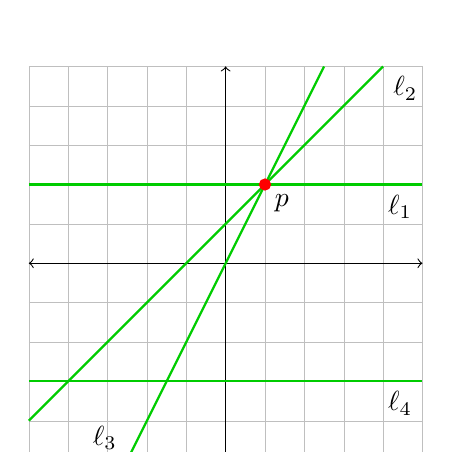
\begin{tikzpicture}%[scale=.9]
    \draw[black, ultra thin] (-2.5,-2.5) rectangle (2.5,2.5);
    \draw[lightgray, ultra thin] (-2.5,-2.5) grid[xstep = 0.5,ystep = 0.5] (2.5,2.5);
    \draw[][->] (0, 0) -- (0, 2.5);
    \draw[][->] (0, 0) -- (2.5, 0);
    \draw[][->] (0, 0) -- (0, -2.5);
    \draw[][->] (0, 0) -- (-2.5, 0);
           
    \draw [green!80!black, thick] (-2.5,1) -- (2.5,1) node[below left,black] {$\ell_1$};
    \draw [green!80!black, thick] (-2.5,-2) -- (2,2.5) node[below right,black] {$\ell_2$};
    \draw [green!80!black, thick] (1.25,2.5) -- (-1.25,-2.5) node[above left,black] {$\ell_3$};
    \draw [green!80!black, thick] (-2.5,-1.5) -- (2.5,-1.5) node[below left,black] {$\ell_4$};
           
    \filldraw [red] (0.5,1) circle (2pt) node[below right,black] {$p$};
  \end{tikzpicture}
 }%
 \qquad
 \subfloat[Dual plane]{
  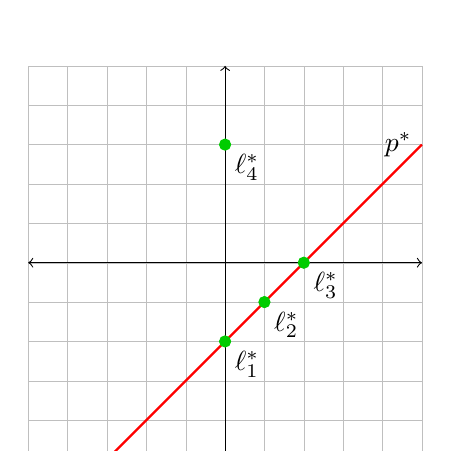
\begin{tikzpicture}%[scale=.9]
    \draw[black, ultra thin] (-2.5,-2.5) rectangle (2.5,2.5);
    \draw[lightgray, ultra thin] (-2.5,-2.5) grid[xstep = 0.5,ystep = 0.5] (2.5,2.5);
    \draw[][->] (0, 0) -- (0, 2.5);
    \draw[][->] (0, 0) -- (2.5, 0);
    \draw[][->] (0, 0) -- (0, -2.5);
    \draw[][->] (0, 0) -- (-2.5, 0);
        
    \draw [red, thick] (-1.5,-2.5) -- (2.5,1.5) node[left,black] {$p^*$};
        
    \filldraw [green!80!black] (0,-1) circle (2pt) node[below right,black] {$\ell_1^*$};
    \filldraw [green!80!black] (0.5,-0.5) circle (2pt) node[below right,black] {$\ell_2^*$};
    \filldraw [green!80!black] (1,0) circle (2pt) node[below right,black] {$\ell_3^*$};
    \filldraw [green!80!black] (0,1.5) circle (2pt) node[below right,black] {$\ell_4^*$};
  \end{tikzpicture}
  }%
  \caption{An example of plane duality.}
  \label{plane_duality_example_figure}
\end{figure}

The duality transform we will use is the following. Let $p:=(p_x,p_y)$ be a point in the plane. The dual of $p$ will be the line $p^*:=(y=p_x \cdot x-p_y)$. The dual of a line $\ell:=(y=m\cdot x+b)$ will be the point $p$ such that $p^*=\ell$, which is $\ell^*:=(m,-b)$.
 
We are interested in certain properties that, if held in the primal plane, also hold in the dual plane. 
  
  %tentei reescrever esses dois aqui de baixo mas nao acho que ficou legal
  
\begin{proposition}\label{dual_lie_proposition}
  A point $p$ lies on a line $\ell$ if and only if the point $\ell^*$ lies on the line~$p^*$.
\end{proposition}
\begin{proof}
  Let $p:=(p_x,p_y)$ and $\ell:=(y=m\cdot x+b)$. Then $p$ lies on $\ell$ if and only if $p_y=m\cdot p_x+b$. 
  We can rewrite that equation to be $-b=p_x \cdot m-p_y$, which means that  $\ell^*:=(m,-b)$ lies on~$p^*:=(y=p_x \cdot x-p_y)$.
\end{proof}
  
\begin{proposition}\label{dual_above_proposition}
  A point $p$ lies above a line $\ell$ if and only if the point $\ell^*$ lies above the line~$p^*$.
\end{proposition}
\begin{proof}
  Let $p:=(p_x,p_y)$ and $\ell:=(y=m\cdot x+b)$. Then $p$ lies above $\ell$ if and only if $p_y>m \cdot p_x+b$. 
  We can rewrite that equation to be $-b>p_x \cdot m-p_y$, which means that  $\ell^*:=(m,-b)$ lies above  $p^*:=(y=p_x \cdot x-p_y)$.
\end{proof}
  
Let us translate some definitions so that we can translate Problem~\ref{ham_sandwich_problem} to its dual version. Firstly, we will define what is a point that is in the median zone of a set of lines, which is the dual of a line bisecting a set of points.
  
\begin{definition}\label{median_zone_definition}
  A point $p$ is said to be in the median zone of a set $H$ of lines 
  if there are no more than $\floor{\frac{|H|}{2}}$ lines above it and no more than $\floor{\frac{|H|}{2}}$ lines below it.
\end{definition}
    
Similarly to the algorithm used to check if a line bisects a set of points, we can write a simple linear-time algorithm to check if a point $p$ is in the median zone of a set $H$ of lines.
    
\begin{algorithm}
\begin{algorithmic}[1]
    \Require{a point $p$ and a set $H$ of lines}
    \Ensure{\textsc{true} if $p$ is in the median zone of $H$ and \textsc{false} otherwise}
    
    \State $below \gets 0$
    \State $above \gets 0$
    \For{each line $h$ in $H$}
        \If{$p.y < h.m \cdot p.x + h.b $} $below \gets below + 1$
        \EndIf
        \If{$p.y > h.m \cdot p.x + h.b$} $above \gets above + 1$
        \EndIf
    \EndFor
    \State \Return $below \leq \frac{|H|}{2}$ \And $above \leq \frac{|H|}{2}$
    \end{algorithmic}
    \caption{\textsc{MedianZone}($p$, $H$)}
    \label{median_zone}
\end{algorithm}

We will also need to define a ham sandwich point, which is the dual of a ham sandwich cut.
    
\begin{definition}\label{ham_sandwich_point_definition}
  A ham sandwich point of two sets $H_1$ and $H_2$ of lines is a point that is in the median zone of $H_1$ and $H_2$ simultaneously.
\end{definition}

With that we can define the dual two-dimensional ham sandwich problem, which is the dual of Problem \ref{ham_sandwich_problem}.
  
\begin{problem}[Dual Two-Dimensional Ham Sandwich Problem]\label{dual_ham_sandwich_problem}
  Given sets $H_1$ and $H_2$ of lines in $\RR^2$, find a ham sandwich point for $H_1$ and $H_2$. 
\end{problem}

  \begin{figure}[htbp]%
    \centering
    \subfloat[]{
        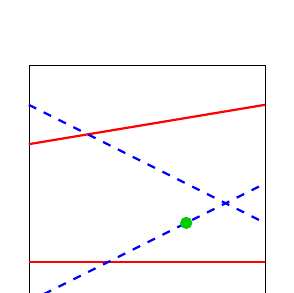
\begin{tikzpicture}
        \draw[black, ultra thin] (0,0) rectangle (3,3);
        
        \draw [red, thick] (0,0.5) -- (3,0.5);
        \draw [red, thick] (0,2) -- (3,2.5);
        
        \draw [blue, thick, dashed] (0,0) -- (3,1.5);
        \draw [blue, thick, dashed] (0,2.5) -- (3,1);
        
        \filldraw [green!80!black] (2,1) circle (2pt);
        \end{tikzpicture}
    }%
    \qquad
    \subfloat[]{
        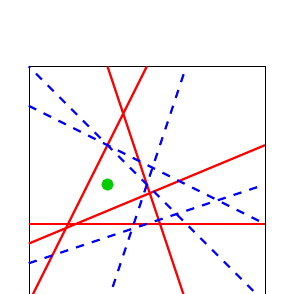
\begin{tikzpicture}
        \draw[black, ultra thin] (0,0) rectangle (3,3);
        
        \draw [red, thick] (0,0) -- (1.5,3);
        \draw [red, thick] (0,0.75) -- (3,2);
        \draw [red, thick] (2,0) -- (1,3);
        \draw [red, thick] (0,1) -- (3,1);
        
        \draw [blue, thick, dashed] (3,0) -- (0,3);
        \draw [blue, thick, dashed] (0,0.5) -- (3,1.5);
        \draw [blue, thick, dashed] (0,2.5) -- (3,1);
        \draw [blue, thick, dashed] (1,0) -- (2,3);
        
        \filldraw [green!80!black] (1,1.5) circle (2pt);
        \end{tikzpicture}
    }%
    \qquad
    \subfloat[]{
        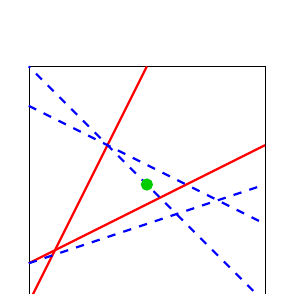
\begin{tikzpicture}
        \draw[black, ultra thin] (0,0) rectangle (3,3);
        
        \draw [red, thick] (0,0) -- (1.5,3);
        \draw [red, thick] (0,0.5) -- (3,2);
        
        \draw [blue, thick, dashed] (3,0) -- (0,3);
        \draw [blue, thick, dashed] (0,0.5) -- (3,1.5);
        \draw [blue, thick, dashed] (0,2.5) -- (3,1);
        
        \filldraw [green!80!black] (1.5,1.5) circle (2pt);
        \end{tikzpicture}
    }%
    \caption{The lines in red (solid) represent $H_1$ and the lines in blue (dashed) represent $H_2$.
    The marked points are solutions to the dual ham sandwich problem for $H_1$ and $H_2$.}%
    \label{dual_ham_sandwich_examples_figure}%
\end{figure}

It can be proven that, if the lines are in general position, such a point always exists, so we would like to find it as efficiently as possible. If there are parallel lines, such point might not exist, which is the case for the examples in Figure \ref{no_answer_example}.

  \begin{figure}[htbp]%
    \centering
    \subfloat[]{
        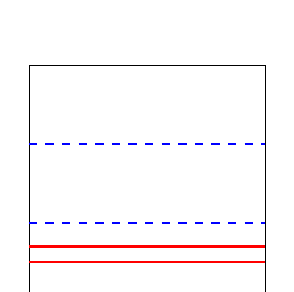
\begin{tikzpicture}
        \draw[black, ultra thin] (0,0) rectangle (3,3);
        
        \draw [red, thick] (0,0.5) -- (3,0.5);
        \draw [red, thick] (0,0.7) -- (3,0.7);
        
        \draw [blue, thick, dashed] (0,2) -- (3,2);
        \draw [blue, thick, dashed] (0,1) -- (3,1);
        
        \end{tikzpicture}
    }%
    \qquad
    \subfloat[]{
        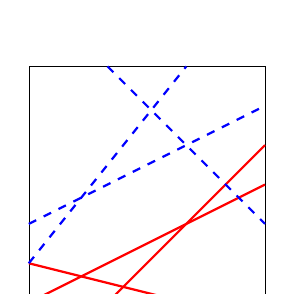
\begin{tikzpicture}
        \draw[black, ultra thin] (0,0) rectangle (3,3);
        
        \draw [red, thick] (0,0) -- (3,1.5);
        \draw [red, thick] (0,0.5) -- (2,0);
        \draw [red, thick] (1,0) -- (3,2);
        
        \draw [blue, thick, dashed] (0,1) -- (3,2.5);
        \draw [blue, thick, dashed] (0,0.5) -- (2,3);
        \draw [blue, thick, dashed] (1,3) -- (3,1);
        
        \end{tikzpicture}
    }%
    \qquad
    \subfloat[]{
        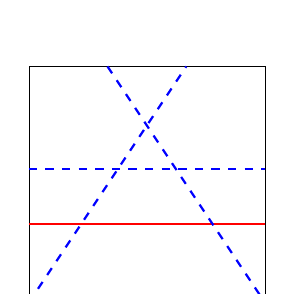
\begin{tikzpicture}
        \draw[black, ultra thin] (0,0) rectangle (3,3);
        
        \draw [red, thick] (0,1) -- (3,1);
        
        \draw [blue, thick, dashed] (0,1.7) -- (3,1.7);
        \draw [blue, thick, dashed] (0,0) -- (2,3);
        \draw [blue, thick, dashed] (1,3) -- (3,0);
        
        \end{tikzpicture}
    }%
    \caption{The lines in red (solid) represent $H_1$ and the lines in blue (dashed) represent $H_2$. There is no ham sandwich point for $H_1$ and $H_2$. }%
    \label{no_answer_example}%
\end{figure}

\begin{proposition}\label{problem_equivalence_proposition}
  In general position, Problem \ref{ham_sandwich_problem} and Problem \ref{dual_ham_sandwich_problem} are equivalent. 
  In other words, a line $\ell$ is a ham sandwich cut for the sets $P_1$ and $P_2$ of points in general position 
  if and only if the point~$\ell^*$ is a ham sandwich point for the sets $P_1^*$ and $P_2^*$ of lines.
\end{proposition}
\begin{proof}
  By Proposition \ref{dual_above_proposition}, a line $\ell$ bisects a set $P$ of points if and only if~$\ell^*$ is in the median zone of $P^*$.
  That way, a line $\ell$ is a ham sandwich cut for the sets $P_1$ and $P_2$ of points if and only if the point $\ell^*$ is a ham sandwich point for the sets $P_1^*$ and~$P_2^*$ of lines.
\end{proof}

To solve Problem \ref{dual_ham_sandwich_problem} in general position, similarly to Problem \ref{ham_sandwich_problem}, we may assume that the number of lines in both sets is odd. That way, the point that corresponds to a solution will be the intersection of a line in $H_1$ and a line in $H_2$.

 \begin{figure}[htbp]%
    \centering
    \subfloat[Primal plane]{
        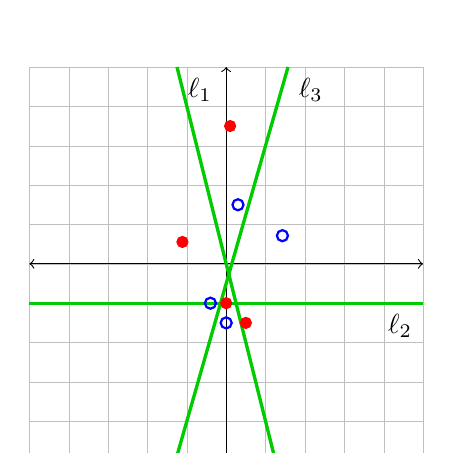
\begin{tikzpicture}
        \draw[black, ultra thin] (-2.5,-2.5) rectangle (2.5,2.5);
        \draw[lightgray, ultra thin] (-2.5,-2.5) grid[xstep = 0.5,ystep = 0.5] (2.5,2.5);
        \draw[][->] (0, 0) -- (0, 2.5);
        \draw[][->] (0, 0) -- (2.5, 0);
        \draw[][->] (0, 0) -- (0, -2.5);
        \draw[][->] (0, 0) -- (-2.5, 0);
        
        \draw [green!80!black, very thick] (5/8,-20/8) -- (-5/8,20/8) node[below right,black] {$\ell_1$};
        \draw [green!80!black, very thick] (-2.5,-0.5) -- (2.5,-0.5) node[below left,black] {$\ell_2$};
        \draw [green!80!black, very thick] (-9/14,-2.5) -- (11/14,2.5) node[below right,black] {$\ell_3$};
        
        \filldraw [red] (1/4,-3/4) circle (2pt) node[below right,black] {};        \filldraw [red] (1/20,7/4) circle (2pt) node[below right,black] {};
        \filldraw [red] (-10/18,5/18) circle (2pt) node[below right,black] {};
        \filldraw [red] (0,-1/2) circle (2pt) node[below right,black] {};
        
        \draw [blue,thick](0,-3/4) circle (2pt) node[below right,black] {};      \draw [blue,thick](-2/10,-0.5) circle (2pt) node[below right,black] {};
        \draw [blue,thick](3/20,3/4) circle (2pt) node[below right,black] {};
        \draw [blue,thick](10/14,5/14) circle (2pt) node[below right,black] {};
        \end{tikzpicture}
    }%
    \qquad
    \subfloat[Dual plane]{
        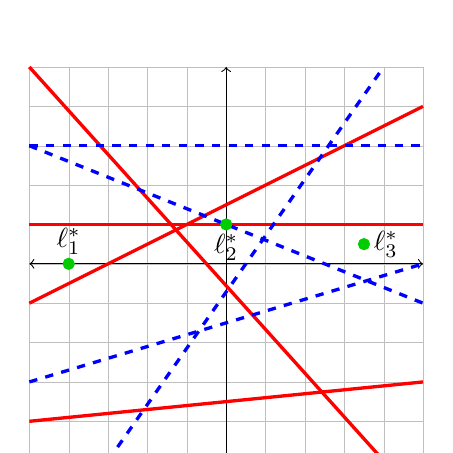
\begin{tikzpicture}
        \draw[black, ultra thin] (-2.5,-2.5) rectangle (2.5,2.5);
        \draw[lightgray, ultra thin] (-2.5,-2.5) grid[xstep = 0.5,ystep = 0.5] (2.5,2.5);
        \draw[][->] (0, 0) -- (0, 2.5);
        \draw[][->] (0, 0) -- (2.5, 0);
        \draw[][->] (0, 0) -- (0, -2.5);
        \draw[][->] (0, 0) -- (-2.5, 0);
        
        \draw [red, very thick] (-2.5,-0.5) -- (2.5,2) node[below left,black] {};
        \draw [red, very thick] (-2.5,-2) -- (2.5,-1.5) node[below left,black] {};
        \draw [red, very thick] (-2.5,2.5) -- (2,-2.5) node[above right,black] {};
        \draw [red, very thick] (-2.5,0.5) -- (2.5,0.5) node[below left,black] {};
        
        \draw [blue, very  thick, dashed] (-2.5,1.5) -- (2.5,1.5) node[below left,black] {};
        \draw [blue, very  thick, dashed] (-2.5,1.5) -- (2.5,-0.5) node[below left,black] {};
        \draw [blue, very  thick, dashed] (-2.5,-1.5) -- (2.5,0) node[below left,black] {};
        \draw [blue, very  thick, dashed] (-1.5,-2.5) -- (2,2.5) node[below right,black] {};
        
        \filldraw [green!80!black] (-2,0) circle (2pt) node[above,black] {$\ell^*_1$};
        \filldraw [green!80!black] (0,0.5) circle (2pt) node[below,black] {$\ell^*_2$};
        \filldraw [green!80!black] (1.75,0.25) circle (2pt) node[right,black] {$\ell^*_3$};
        \end{tikzpicture}
    }%
    \caption{The same instance of the ham sandwich problem both in the primal and in the dual plane. 
             For $1\leq i \leq 3$, line $\ell_i$ and point $\ell^*_i$ represent possible solutions in their respective planes.}
    \label{ham_sandwich_translation_figure}
\end{figure}

That gives us a naive solution to Problem \ref{dual_ham_sandwich_problem}, presented in Algorithm~\ref{dual_n3_algorithm}: go through all intersections of two lines and check if each intersection is a ham sandwich point.

\begin{algorithm}
\begin{algorithmic}[1]
\Require{two nonempty sets $H_1$ and $H_2$ of lines in general position}
\Ensure{a ham sandwich point $p$ of $H_1$ and $H_2$}

 \For{each line $h_1$ in $H_1$}
  \For{each line $h_2$ in $H_2$}
    \State $x \gets \frac{h_2.b - h_1.b}{h_1.m - h_2.m}$
    \State $y \gets h_1.m \cdot x +h_1.b $
    \State $p \gets (x,y)$  \hfill {\small \textcolor{gray}{$\rhd$ intersection of $h_1$ and $h_2$}}
    \If{\textsc{MedianZone}($p$, $H_1$) \And \textsc{MedianZone}($p$, $H_2$)} \Return{$p$}
    \EndIf
  \EndFor
 \EndFor
\end{algorithmic}
\caption{\textsc{DualNaiveSolve}($H_1$, $H_2$)}
\label{dual_n3_algorithm}
\end{algorithm}

Algorithm~\ref{dual_n3_algorithm} just happens to be Algorithm~\ref{n3_algorithm} converted to the dual plane.
It can also be optimized to run in $\bigo(n^2 \log n)$ time (where $n:=|H_1|+|H_2|$), but, in the dual plane, the optimized version, shown in Algorithm~\ref{dual_n2log_algorithm}, is a sweep line algorithm that is much easier to visualize.

The algorithm sweeps the plane from left to right, keeping the order in which the red and the blue lines intersect the sweep line. Initially, the lines intersect the sweep line in order of their slopes.  This order changes every time the sweep line passes by an  intersection of two lines of the same color.  Intersections of two lines of different color are candidates to ham sandwich points, so the events of this sweep line algorithm are the intersections of pairs of the given lines.  These intersections are processed in order of their x-coordinate. 

Intersections of lines of the same color cause the order of the intersection of these lines with 
the sweep line to invert.  Intersections of lines of different color are tested to see if they are a ham sandwich point. 
For this test to be made efficiently, the algorithm keeps track of the position of each line in the order of intersection of 
all lines of its color with the sweep line.  To decide whether an intersection of two lines of different color is a ham sandwich 
point, it is enough to check whether both lines are in the middle position of their respective color order. 

\newcommand{\IntersectionSort}{\textsc{IntersectionSort}}
\newcommand{\SlopeSort}{\textsc{SlopeSort}}
\newcommand{\IdPerm}{\textsc{IdentityPermutation}}

In Algorithm~\ref{dual_n2log_algorithm}, the procedure $\SlopeSort(H)$ sorts the list $H$ of lines by slope and the procedure $\IdPerm(n)$ returns the identity permutation of the integers between 1 and $n$.
The first runs in $\bigo(n \log n)$, where $n = |H|$, and the second runs in $\bigo(n)$.
The procedure $\IntersectionSort(H_1,H_2)$ receives two sets $H_1$ and $H_2$ of lines in general position and returns a list of all pairs of lines in~$H_1 \cup H_2$ that intersect, sorted by the $x$-coordinate of the intersection.  Each line is identified by an integer $i$ in $\{1,2\}$ and the index of the line in $H_i$.  This procedure runs in $\bigo(n^2 \log n)$, where $n = |H_1| + |H_2|$.

\newcommand{\Events}{\mathit{Events}}

\begin{algorithm}
\begin{algorithmic}[1]
 \Require{two nonempty sets $H_1$ and $H_2$ of lines in general position}
 \Ensure{a ham sandwich point $p$ of $H_1$ and $H_2$}

 \If{$|H_1|$ is even} remove an arbitrary line of $H_1$
 \EndIf
 \If{$|H_2|$ is even} remove an arbitrary line of $H _2$
 \EndIf
 \State $\SlopeSort(H_1)$ \hfill {\small \textcolor{gray}{$\rhd$ $H_1[1].m < \cdots < H_1[|H_1|].m$}}
 \State $\pi_1 \gets \IdPerm(|H_1|)$
 \State $\SlopeSort(H_2)$ \hfill {\small \textcolor{gray}{$\rhd$ $H_2[1].m < \cdots < H_2[|H_2|].m$}}
 \State $\pi_2 \gets \IdPerm(|H_2|)$
 \State \hfill {\small \textcolor{gray}{$\rhd$ Order of the intersection with the sweep line: $H_i[\pi_i[1]] \prec \cdots \prec H_i[\pi_i[|H_i|]]$ for $i = 1,2$}}
 \State $\Events \gets \IntersectionSort(H_1,H_2)$
 \State $t_1 \gets \ceil{\frac{|H_1|}2}$
 \State $t_2 \gets \ceil{\frac{|H_2|}2}$
 \For{each $\{(i,j), (i',j')\}$ in $Events$}
    \If {$i = i'$} \hfill {\small \textcolor{gray}{$\rhd$ both lines are in the same $H_i$?}}
    \State $H_i[\pi_i[j]] \leftrightarrow H_i[\pi_i[j']]$
    \State $\pi_i[j] \leftrightarrow \pi_i[j']$ 
                   \hfill {\small \textcolor{gray}{$\rhd$ they exchange places in the order $\prec$}}
    \Else \hfill {\small \textcolor{gray}{$\rhd$ check whether the intersection is a ham sandwich point}}
       \If{$\pi_i[j] = t_i$ \And $\pi_{i'}[j'] = t_{i'}$} \hfill {\small \textcolor{gray}{$\rhd$ both lines are in the median level?}}
          \State $x \gets \frac{H_1[t_1].b - H_2[t_2].b}{H_2[t_2].m - H_1[t_1].m}$
          \State $y \gets H_1[t_1].m \ x + H_2[t_2].b$ \hfill {\small \textcolor{gray}{$\rhd$ their intersection}}
          \State \Return $(x,y)$
       \EndIf
    \EndIf
  \EndFor
\end{algorithmic}
\caption{\textsc{OptimizedDualNaiveSolve}($H_1$, $H_2$)}
\label{dual_n2log_algorithm}
\end{algorithm}

The complexity of Algorithm~\ref{dual_n2log_algorithm} is that of $\IntersectionSort(H_1,H_2)$, that is, $\bigo(n^2 \log n)$.

\newpage
\subsection{Existence}\label{sec:existence}

The duality transformation also makes it easier to prove that there is always a solution to the ham sandwich problem.

Firstly, we will assume that the points in $P_1$ and $P_2$ are in general position, which implies that every pair of lines in $P_1^*$ and $P_2^*$ intersects at exactly one point and there are no vertical lines.  % We will also assume that both $|P_1|$ and $|P_2|$ are odd.

To prove the existence of a ham sandwich cut, we will need to make some observations:

\begin{proposition}
\label{median_level_preposition}
The median zone of an odd set of lines is a polygonal chain.
\end{proposition}
\begin{proof}
Let $H$ be an odd set of lines.
Because $|H|$ is odd, for a point to be below $\floor{\frac{|H|}{2}}$ lines and above $\floor{\frac{|H|}{2}}$ lines, it must lay on a line of $H$. Furthermore, most of the times there is only one candidate for which line of $H$ that point must lay on given its x-coordinate: the line that is in the middle when we sort $H$ by the intersection with the vertical line that passes by the point.

Notice that the line that represents the median zone only changes when that line intersects with the next median line, that other line will now be the one to represent the median zone.
That means that the median zone is a connected series of line segments, i.e., a polygonal chain.
\end{proof}

\begin{definition}\label{level_definition}
  The $i$-th level of a set $H$ of lines, denoted as $L_i(H)$, is the polygonal chain such that there are exactly $i-1$ lines of~$H$ strictly below $L_i(H)$ and exactly $|H|-i$ lines of~$H$ strictly above $L_i(H)$
\end{definition}

Note that the median level of an odd set $H$ of lines, $L_{\ceil{\frac{|H|}{2}}}(H)$, is the median zone of~$H$.

 \begin{figure}[!htbp]%
    \centering

    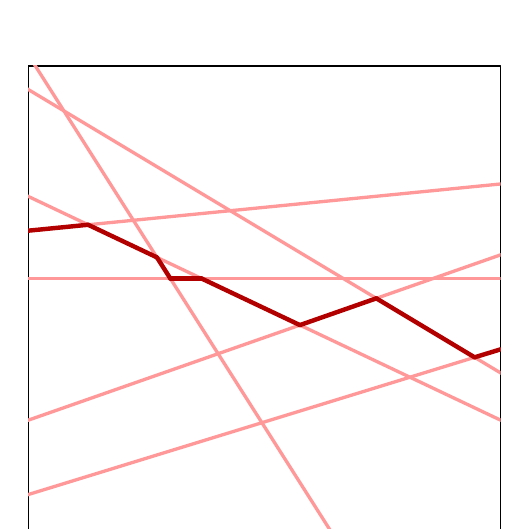
\begin{tikzpicture}[line cap=round,line join=round,>=triangle 45,x=1cm,y=1cm]
    \begin{axis}[
    ticks=none,
    x=1.5cm,y=1.5cm,
    %ymajorgrids=true,
    %xmajorgrids=true,
    xmin=-2,
    xmax=2,
    ymin=-2,
    ymax=2,]
    \clip(-2,-2) rectangle (2,2);
    
    \draw[black, ultra thin] (-2,-2) rectangle (2,2);
    \draw [red!40!white, very thick, domain=-3.6910139103109825:7.605061386513559] plot(\x,{(-0.2-1.8*\x)/3.8});
    \draw [red!40!white, very thick, domain=-3.6910139103109825:7.605061386513559] plot(\x,{(-1.2--1.4*\x)/4});
    \draw [red!40!white, very thick, domain=-3.6910139103109825:7.605061386513559] plot(\x,{(-2.527913809990206-3.772771792360431*\x)/2.3957884427032323});
    \draw [red!40!white, very thick, domain=-3.6910139103109825:7.605061386513559] plot(\x,{(-4.05575923654655--1.2285602707581362*\x)/3.9965967375756906});
    \draw [red!40!white, very thick, domain=-3.6910139103109825:7.605061386513559] plot(\x,{(-1.04-0*\x)/-5.2});
    \draw [red!40!white, very thick, domain=-3.6910139103109825:7.605061386513559] plot(\x,{(-2.4--2.4*\x)/-4});
    \draw [red!40!white, very thick, domain=-3.6910139103109825:7.605061386513559] plot(\x,{(--3.5235261518335377--0.43440500611541055*\x)/4.392336164064359});
    \draw[red!70!black, ultra thick]  (-2.392336164064359,0.5655949938845894) -- (-1.49293188625848,0.6545466829645432);
    \draw[red!70!black, ultra thick]  (-1.49293188625848,0.6545466829645432) -- (-0.9104959441581613,0.37865597354860275);
    \draw[red!70!black, ultra thick]  (-0.9104959441581613,0.37865597354860275) -- (-0.7970456905503636,0.2);
    \draw[red!70!black, ultra thick]  (-0.7970456905503636,0.2) -- (-0.5333333333333332,0.2);
    \draw[red!70!black, ultra thick]  (-0.5333333333333332,0.2) -- (0.3003194888178914,-0.19488817891373805);
    \draw[red!70!black, ultra thick]  (0.3003194888178914,-0.19488817891373802) -- (0.9473684210526317,0.03157894736842107);
    \draw[red!70!black, ultra thick]  (0.9473684210526317,0.03157894736842107) -- (1.779287316474339,-0.46757238988460326);
    \draw[red!70!black, ultra thick]  (1.779287316474339,-0.46757238988460326) -- (2.025452796577689,-0.3921757693587057);
    \end{axis}
    \end{tikzpicture}
\caption{The darker polygonal chain represents the median level of the set of lines displayed.}
\end{figure}

Now let $P_1$ and $P_2$ be the sets of points in general position for which we want to find a ham sandwich cut. We are looking for a line that bisects both $P_1$ and $P_2$, which is the same as a point that is in the median zone of both $P_1^*$ and $P_2^*$. If $P_1$ and $P_2$ are odd, that means we want to find an intersection of the median levels of both. If that intersection exists, then it is an answer to the original problem.

\begin{lemma}
\label{odd_intersection_lemma}
Let $H_1$ and $H_2$ be two odd sets of lines in general position. Their median levels intersect at an odd number of points.
\end{lemma}
\begin{proof}
    The left unbounded ray and the right unbounded ray of the median level of any odd set of lines in general position lie on the same line: the line that is the median in the slope order. Let us say such line is $h_1$ for $H_1$ and  $h_2$ for $H_2$. Because the lines are in general position, one of them must have a smaller slope. Let us assume without loss of generality that this is $h_1$.
    
    That means that, for small enough $x$, $h_1(x)>h_2(x)$ and the median level of $H_1$ is above the median level of $H_2$ and, for large enough $x$, $h_1(x)<h_2(x)$ and the median level of $H_1$ is below the median level of $H_2$. By continuity, the median levels intersect an odd number of times. 
\end{proof}

\begin{figure}[!htbp]%
    \centering
    \subfloat[]{
        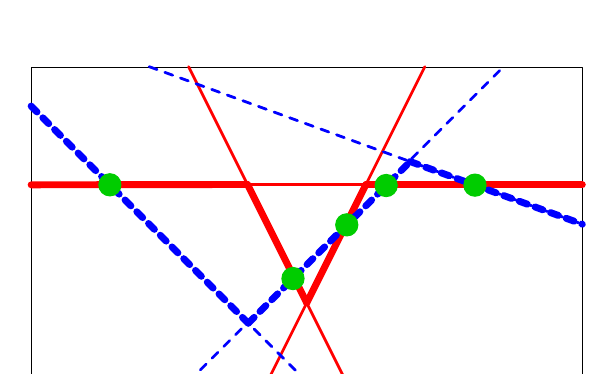
\begin{tikzpicture}[line cap=round,line join=round,>=triangle 45,x=1cm,y=1cm]
        \draw[black, ultra thin] (-7/2,-4/2) rectangle (7/2,4/2);
            
    \draw [line width=1pt,red] (-7/2,1/2) -- (7/2,1/2);
    \draw [line width=1pt,red] (-3/2,4/2) -- (1/2,-4/2);
    \draw [line width=1pt,red] (-1/2,-4/2) -- (3/2,4/2);
    \draw [line width=1pt,blue,dashed] (-3/2,-4/2) -- (5/2,4/2);
    \draw [line width=1pt,blue,dashed] (-4/2,4/2) -- (7/2,0/2);
    \draw [line width=1pt,blue,dashed] (-7/2,3/2) -- (0,-4/2);
    \draw [line width=2.5pt,red] (-7/2,1/2) -- (-1.504/2,1.008/2);
    \draw [line width=2.5pt,red] (-1.504/2,1.008/2) -- (0,-2/2);
    \draw [line width=2.5pt,red] (0,-2/2) -- (1.5/2,1/2);
    \draw [line width=2.5pt,red] (1.5/2,1/2) -- (7/2,1/2);
    \draw [line width=2.5pt,blue,dashed] (-7/2,3/2) -- (-1.485/2,-2.515/2);
    \draw [line width=2.5pt,blue,dashed] (-1.485/2,-2.515/2) -- (2.6272992700729922/2,1.5900729927007298/2);
    \draw [line width=2.5pt,blue,dashed] (2.6272992700729927/2,1.59007299270073/2) -- (7/2,0/2);
    
    \filldraw [green!80!black] (-5/2,1/2) circle (4pt);
    \filldraw [green!80!black] (-0.34899396888982054/2,-1.380990198769563/2) circle (4pt);
    \filldraw [green!80!black] (1.01718333826261/2,-0.01721358658430571/2) circle (4pt);
    \filldraw [green!80!black] (2.0180619545452707/2,0.9819062504796678/2) circle (4pt);
    \filldraw [green!80!black] (4.2732846715328465/2,0.9915328467153284/2) circle (4pt);
    
    \end{tikzpicture}
    }%
    \qquad
    \subfloat[]{
        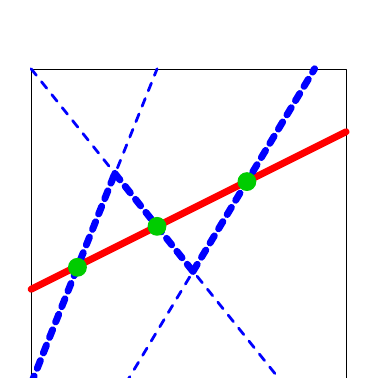
\begin{tikzpicture}[scale=.8,line cap=round,line join=round,>=triangle 45,x=1cm,y=1cm]
        \draw[black, ultra thin] (-5/2,-5/2) rectangle (5/2,5/2);
                
        \draw [line width=2.5pt,red] (-2.5,-1) -- (2.5,1.5);
        \draw [line width=1pt,blue,dashed] (-2.5,-2.5) -- (-0.5,2.5);
        \draw [line width=1pt,blue,dashed] (-2.5,2.5) -- (1.5,-2.5);
        \draw [line width=1pt,blue,dashed] (-1,-2.5) -- (2,2.5);
        \draw [line width=2.5pt,blue,dashed] (-2.5,-2.5) -- (-1.1715447154471537,0.8394308943089421);
        \draw [line width=2.5pt,blue,dashed] (-1.1715447154471537,0.8394308943089422) -- (0.06921568627451036,-0.7179738562091494);
        \draw [line width=2.5pt,blue,dashed] (0.0692156862745103,-0.7179738562091496) -- (2,2.5);
        
        
        
        \filldraw [green!80!black] (-1.7645707618889337,-0.6513001251277831) circle (4pt);
        \filldraw [green!80!black]  (-0.5017024695714511,-0.0013563313125183995) circle (4pt);
        \filldraw [green!80!black]  (0.9252941176470592,0.708823529411765) circle (4pt);
        
        \end{tikzpicture}
    }%
    \caption{Some examples of the odd intersection property. The red (solid) lines represent~$H_1$, the blue (dashed) lines represent~$H_2$. The thicker lines represent the median level of each set and the points represent where those median levels intersect.}
    \label{odd_intersection_examples_picture}
\end{figure}

If the set of lines is not in general position the lines the median levels lay on might be parallel. In those cases, the median level of the two sets of lines do not necessarily intersect and there might be no solution for the problem as stated.

\begin{figure}[!htbp]%
    \centering
    \subfloat[]{
    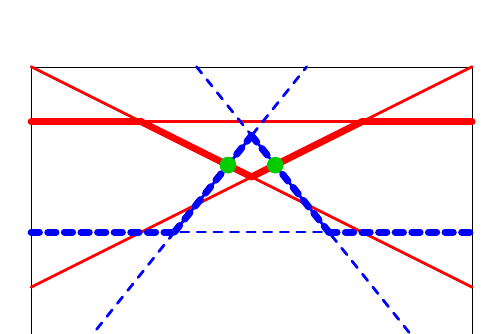
\begin{tikzpicture}[scale=.7,line cap=round,line join=round,>=triangle 45,x=1cm,y=1cm]
    \draw[black, ultra thin] (-4,-1) rectangle (4,4);
    \draw [line width=1pt,red] (-4,3)-- (4,3);
    \draw [line width=1pt,red] (-4,4)-- (4,0);
    \draw [line width=1pt,red] (-4,0)-- (4,4);
    \draw [line width=2.5pt,red] (-4,3)-- (-2,3);
    \draw [line width=2.5pt,red] (-2,3)-- (0,2);
    \draw [line width=2.5pt,red] (0,2)-- (2,3);
    \draw [line width=2.5pt,red] (2,3)-- (4,3);
    \draw [line width=1pt,blue,dashed] (-4,1)-- (4,1);
    \draw [line width=1pt,blue,dashed] (-3,-1)-- (1,4);
    \draw [line width=1pt,blue,dashed] (-1,4)-- (3,-1);
    \draw [line width=2.5pt,blue,dashed] (-4,1)-- (-1.4,1);
    \draw [line width=2.5pt,blue,dashed] (-1.4,1)-- (0,2.75);
    \draw [line width=2.5pt,blue,dashed] (0,2.75)-- (1.4,1);
    \draw [line width=2.5pt,blue,dashed] (1.4,1)-- (4,1);
    \filldraw [green!80!black] (-0.42876381382059625,2.2143819069102983) circle (4pt);
    \filldraw [green!80!black] (0.4285726080237532,2.214286304011877) circle (4pt);
    \end{tikzpicture}
    }%
    \qquad
    \subfloat[]{
        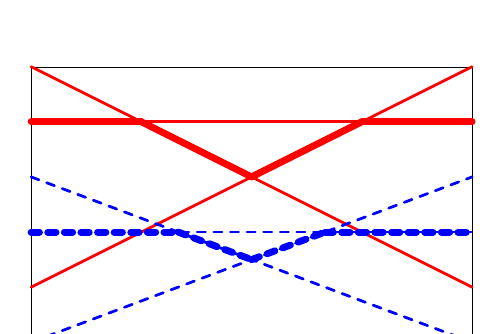
\begin{tikzpicture}[scale=.7,line cap=round,line join=round,>=triangle 45,x=1cm,y=1cm]
        \draw[black, ultra thin] (-4,-1) rectangle (4,4);
        \draw [line width=1pt,red] (-4,3)-- (4,3);
        \draw [line width=1pt,red] (-4,4)-- (4,0);
        \draw [line width=1pt,red] (-4,0)-- (4,4);
        \draw [line width=2.5pt,red] (-4,3)-- (-2,3);
        \draw [line width=2.5pt,red] (-2,3)-- (0,2);
        \draw [line width=2.5pt,red] (0,2)-- (2,3);
        \draw [line width=2.5pt,red] (2,3)-- (4,3);
        \draw [line width=1pt,blue,dashed] (-4,1)-- (4,1);
        \draw [line width=1pt,blue,dashed] (-4,2)-- (4,-1);
        \draw [line width=1pt,blue,dashed] (-4,-1)-- (4,2);
        \draw [line width=2.5pt,blue,dashed] (-4,1)-- (-1.3333333333333333,1);
        \draw [line width=2.5pt,blue,dashed] (-1.3333333333333333,1)-- (0,0.5);
        \draw [line width=2.5pt,blue,dashed] (0,0.5)-- (1.3333333333333333,1);
        \draw [line width=2.5pt,blue,dashed] (1.3333333333333333,1)-- (4,1);
        
        \end{tikzpicture}
    }%
    \caption{When the median levels of the sets of lines are parallel, their median levels may or may not intersect.}
    \label{odd_intersection_examples_picture}
\end{figure}

Now we can finally prove the result.

\begin{theorem}
    Given two sets $P_1$ and $P_2$ of points in $\realnumbers^2 $ in general position, there always exists a line that bisects both sets simultaneously.
\end{theorem}
\begin{proof}
By Proposition \ref{can_solve_odd_proposition} we may assume both sets of points are odd, as otherwise we can just remove any point from the even sets and the solution found will still be applicable.

By Proposition \ref{problem_equivalence_proposition}, it is enough to find a ham sandwich point $p$ for $H_1:=P_1^*$ and $H_2:=P_2^*$.

From Lemma \ref{odd_intersection_lemma}, the median levels of $H_1$ and $H_2$ intersect an odd number of times, which is necessarily a positive number of times. That means there is a point $p$ that is in both the median level of $H_1$ and in the median level of $H_2$, so $p$ is a ham sandwich point, and therefore, our solution.

\end{proof}

\newpage
\section{The Algorithm}\label{sec:nlogn}

We will now outline the basic steps in the $\bigo(n)$ solution, where $n:=|H_1|+|H_2|$, for Problem~\ref{dual_ham_sandwich_problem} and, because of Proposition \ref{problem_equivalence_proposition}, for Problem \ref{ham_sandwich_problem}. We will also detail an implementation of an~$\bigo(n \log n)$ algorithm that shares those same basic steps.

In Section \ref{sec:linear} we will go over what are the changes that will be needed for the $\bigo(n \log n)$ algorithm to turn into the $\bigo(n)$ one we are looking for.

The $\bigo(n)$ algorithm was first described in [1]. There you can also find a proof for its correctness. Here we will outline the same steps that were described in that article and fill in some of the implementation details.\\

The algorithm will search for an intersecction between the median zones of our two sets of lines, $H_1$ and $H_2$. In our description, we will use the following:

\begin{definition}
Let $T$ be an interval. A \textit{$T$-intersection} is an intersection between two lines whose $x$-coordinate lies in~$T$.
\end{definition}

\begin{definition}
Let $T$ be an interval. A \textit{T-trapezoid} is a trapezoid that has two sides parallel to the $y$-axis, the first of which is a segment contained in the vertical line defined by the beginning of $T$ and the second of which is a segment contained in the vertical line defined by the end of $T$.
\end{definition}

\begin{definition}
Let $T$ be an interval, $G_1$ and $G_2$ sets of lines and $p_1$ and $p_2$ integers such that $1 \leq p_i \leq |G_i|$. $T$ has the odd intersection property in relation to $L_{p_1}(G_1)$ and $L_{p_2}(G_2)$ if $L_{p_1}(G_1)$ and $L_{p_2}(G_2)$ intersect an odd number of times in $T$.
\end{definition}

The basic idea of the algorithm is to find subsets $G_1$ and $G_2$ of $H_1$ and $H_2$, respectively, in such a way that there is at least one intersection of the median levels of $H_1$ and $H_2$ that is also an intersection of a line in~$G_1$ and a line in $G_2$. We will be removing lines from $G_1$ and $G_2$ in phases while maintaining this property, and once $|G_1|+|G_2|$ is small enough, we will find a solution using some naive algorithm.

The algorithm will work in phases. At the beginning of each phase, the algorithm will have the following data:

\begin{itemize}
    \item an open interval $T$ on the $x$-axis that has the odd intersection property in relation to $L_{p_1}(G_1)$ and $L_{p_2}(G_2)$;
    \item current sets $G_1$ and $G_2$ of lines, $G_i \subseteq H_i$;
    \item  integers $p_1$ and $p_2$, $1 \leq p_i \leq |G_i|$ such that all $T$-intersections between $L_{p_1}(G_1)$ and $L_{p_2}(G_2)$ are valid ham-swandwich points por $H_1$ and $H_2$.
\end{itemize}

At the end of the phase, lines have been discarded so we now have new sets $G_i' \subseteq G_i$, integers $p_i'$ such that $1 \leq p_i' \leq |G_i'|$, and a new interval $T'\subset T$ on which the invariant holds for the new data.

It is also worth noting that, in the algorithms that will be described in this section, we always assume the lines to be in general position.

To start the algorithm, $T$ is the whole $x$-axis,
$G_i = H_i$ and $p_i = \ceil{\frac{|H_i|}{2}}$.\\

To perform one of the phases, we will execute the following steps, always ensuring beforehand that $|G_1|\geq|G_2|$:

\begin{enumerate}
\item Find an interval $T'\subset T$ such that there are no more than  $\alpha \times {|G_1| \choose 2}$ $T'$-intersections among the lines in $G_1$ and that has the odd intersection property in relation to $L_{p_1}(G_1)$ and $L_{p_2}(G_2)$. Let $T'$ be the new $T$.

This step will be represented by the function \textsc{NewInterval}$(G_1,G_2,p_1,p_2,T)$, which returns the new interval $T'$ given the parameters as stated above.

\item Construct a $T$-trapezoid $\tau$ that contains the entirety of $L_{p_1}(G_1)$ in $T$. We also need to choose $\tau$ in such a way that only a certain predetermined fraction of lines in $G_1$ intersect $\tau$. This fraction is determined by $\alpha$ and its value is such that a $\tau$ as described above always exists. 

This step will be represented by the function \textsc{FindTrapezoid}$(G_1,p_1,T)$, which returns the $T$-trapezoid $\tau$ as per the constraints above.

\item Discard all the lines in $G_1$ that do not intersect $\tau$ and update $p_1$ accordingly.

This step will be represented by the function \textsc{DiscardLines}$(G_1,p_1,\tau)$, which modifies $G_1$ and $p_1$ according to what was described.


\end{enumerate}

If we use $\alpha=\frac{1}{32}$, in the end of the phase, $G_1$ will have its size cut by at least half \cite[Lemma 3.5]{LoMS1994}. Once the size of $G_1$ is smaller than some constant, we can use some naive algorithm to find an $T$-intersection of $L_{p_1}(G_1)$ and $L_{p_2}(G_2)$. This algorithm will be \textsc{BruteForce}$(G_1,G_2,p_1,p_2,T)$.

Since $|G_1|\geq|G_2|$ and $|G_1|$ decreases by half by the end of each phase, $|G_1|+|G_2|$ decreases to at most $\frac{3}{4}$ of its previous value by the end of each phase. If each phase takes time $\bigo(|G_1|+|G_2|)$, the total time for this procedure will be a geometric progression that adds up to $\bigo(|H_1|+|H_2|)=\bigo(n)$.

The final algorithm will be as follows:

%arrumar a constante

\begin{algorithm}
\begin{algorithmic}[1]
\Require{two nonempty sets $G_1$ and $G_2$ of lines}
\Ensure{a point that is in the intersection of the median zones of $G_1$ and $G_2$}
\State $\alpha \gets \frac{1}{32}$
\If{$|G_1|$ is even} remove any line from $G_1$
\EndIf
\If{$|G_2|$ is even} remove any line from $G_2$
\EndIf
\State $p_1 \gets \ceil{\frac{|G_1|}{2}}$
\State $p_2 \gets \ceil{\frac{|G_2|}{2}}$
\State $T \gets (-\infty,\infty)$
\State $T' \gets$ \textsc{NewInterval}$(G_1,G_2,p_1,p_2,T)$
\While{${|G_1|\choose 2}>\frac{1}{\alpha} \ \And \ {|G_2|\choose 2}>\frac{1}{\alpha}$}
\If{$|G_2|>|G_1|$} \hfill {\small \textcolor{gray}{$\rhd$ ensuring $|G_1|\geq|G_2|$}}
\State $G_1\leftrightarrow G_2$
\State $p_1\leftrightarrow p_2$
\EndIf
\State $T \gets T'$
\State $\tau \gets $\textsc{FindTrapezoid}$(G_1,p_1,T)$
\State \textsc{DiscardLines}$(G_1,p_1,\tau)$
\State $T' \gets$ \textsc{NewInterval}$(G_1,G_2,p_1,p_2,T)$
\EndWhile
\State \Return \textsc{BruteForce}$(G_1,G_2,p_1,p_2,T)$ \hfill {\small \textcolor{gray}{$\rhd$ $|G_1|$ and $|G_2|$ are sufficiently small}}
\end{algorithmic}
\caption{\textsc{HamSandwichPoint}($G_1,G_2$)}
\label{ham_sandwich_point_algorithm}
\end{algorithm}

The following figures represent what one of the phases of the algorithm might look like. Here we use an $\alpha$ greater than $\frac{1}{32}$ to make it easier to visualize the lines. As a consequence, less than half the lines will be discarded in Step 3.

\begin{figure}[!htbp]%
\centering
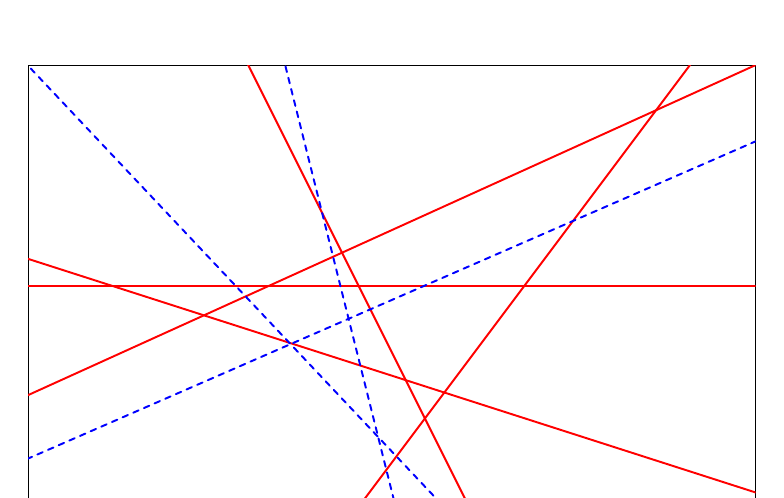
\begin{tikzpicture}[scale=.7,line cap=round,line join=round,>=triangle 45,x=2cm,y=2cm]
\begin{axis}[x=4cm,y=4cm,ticks=none,xmin=-1.5,xmax=1.8,ymin=-1,ymax=1,xtick={},ytick={}]
\draw [line width=1pt,color=red,domain=-5.181742519593772:5.231034803725047] plot(\x,{(-0-0*\x)/4});
\draw [line width=1pt,color=red,domain=-5.181742519593772:5.231034803725047] plot(\x,{(-1.427205958142864-1.280727334321566*\x)/3.988660626785996});
\draw [line width=1pt,color=red,domain=-5.181742519593772:5.231034803725047] plot(\x,{(--0.704763751166452--1.7164128048552574*\x)/3.7835708350505004});
\draw [line width=1pt,color=red,domain=-5.181742519593772:5.231034803725047] plot(\x,{(-0-2*\x)/1});
\draw [line width=1pt,color=red,domain=-5.181742519593772:5.231034803725047] plot(\x,{(-1.5--2*\x)/1.5});

\draw [line width=1pt,color=blue,dashed,domain=-4.308895283329108:4.034134313210317] plot(\x,{(-1.117461907692587-2.0058127146687443*\x)/1.8912571643105291});
\draw [line width=1pt,color=blue,dashed,domain=-4.308895283329108:4.034134313210317] plot(\x,{(-0.5131402247935166--1.7489144866629978*\x)/4.010969198119512});
\draw [line width=1pt,color=blue,dashed,domain=-4.308895283329108:4.034134313210317] plot(\x,{(--0.1335014748795273--1.6047234501056908*\x)/-0.401180862526424});
\end{axis}
\end{tikzpicture}
\caption*{An instance of the Dual 2D Ham Sandwich Problem: \\
the lines in red (solid) represent $H_1$ and the lines in blue (dashed) represent $H_2$.}
\end{figure}
\begin{figure}[!htbp]%
\centering
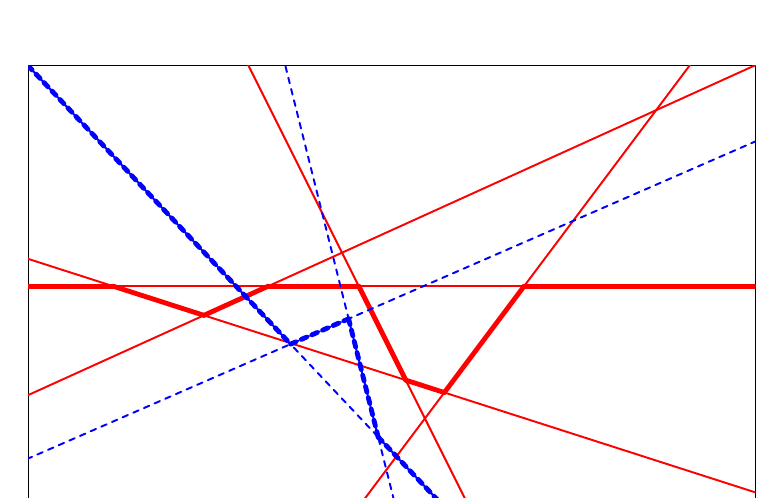
\begin{tikzpicture}[scale=.7,line cap=round,line join=round,>=triangle 45,x=2cm,y=2cm]
\begin{axis}[x=4cm,y=4cm,ticks=none,xmin=-1.5,xmax=1.8,ymin=-1,ymax=1,xtick={},ytick={}]
\draw [line width=1pt,color=red,domain=-5.181742519593772:5.231034803725047] plot(\x,{(-0-0*\x)/4});
\draw [line width=1pt,color=red,domain=-5.181742519593772:5.231034803725047] plot(\x,{(-1.427205958142864-1.280727334321566*\x)/3.988660626785996});
\draw [line width=1pt,color=red,domain=-5.181742519593772:5.231034803725047] plot(\x,{(--0.704763751166452--1.7164128048552574*\x)/3.7835708350505004});
\draw [line width=1pt,color=red,domain=-5.181742519593772:5.231034803725047] plot(\x,{(-0-2*\x)/1});
\draw [line width=1pt,color=red,domain=-5.181742519593772:5.231034803725047] plot(\x,{(-1.5--2*\x)/1.5});
\draw [line width=2.5pt,color=red] (-2,0)-- (-1.1143714355865542,0);
\draw [line width=2.5pt,color=red] (-1.1143714355865542,0)-- (-0.7022802713912073,-0.13231920877727113);
\draw [line width=2.5pt,color=red] (-0.7022802713912073,-0.13231920877727113)-- (-0.4106027111734835,0);
\draw [line width=2.5pt,color=red] (-0.4106027111734835,0)-- (0,0);
\draw [line width=2.5pt,color=red] (0,0)-- (0.21312416063338305,-0.4262483212667661);
\draw [line width=2.5pt,color=red] (0.21312416063338305,-0.4262483212667661)-- (0.3881614448825161,-0.48245140682331183);
\draw [line width=2.5pt,color=red] (0.3881614448825161,-0.48245140682331183)-- (0.75,0);
\draw [line width=2.5pt,color=red] (0.75,0)-- (2,0);

\draw [line width=1pt,color=blue,dashed,domain=-4.308895283329108:4.034134313210317] plot(\x,{(-1.117461907692587-2.0058127146687443*\x)/1.8912571643105291});
\draw [line width=1pt,color=blue,dashed,domain=-4.308895283329108:4.034134313210317] plot(\x,{(-0.5131402247935166--1.7489144866629978*\x)/4.010969198119512});
\draw [line width=1pt,color=blue,dashed,domain=-4.308895283329108:4.034134313210317] plot(\x,{(--0.1335014748795273--1.6047234501056908*\x)/-0.401180862526424});
\draw [line width=2.5pt,color=blue,dashed] (-1.5,1)-- (-0.30931525374422464,-0.2628058459054822);
\draw [line width=2.5pt,color=blue,dashed] (-0.30931525374422464,-0.2628058459054822)-- (-0.046175733411063916,-0.14806836067623147);
\draw [line width=2.5pt,color=blue,dashed] (-0.046175733411063916,-0.14806836067623147)-- (0.08780119683678558,-0.6839760816676277);
\draw [line width=2.5pt,color=blue,dashed] (0.08780119683678558,-0.6839760816676277)-- (0.3912571643105291,-1.0058127146687441);
\end{axis}
\end{tikzpicture}
\caption*{The parameters at the beginning of the algorithm: $T$ is the whole $x$-axis, $G_1 = H_1$, $G_2 = H_2$, $p_1 = 3$ and $p_2 = 2$. The thicker lines show the levels $L_{p_1}(G_1)$ and $L_{p_2}(G_2)$.} 
\end{figure}

\begin{figure}[!htbp]%
\centering
\begin{tikzpicture}[scale=.7,line cap=round,line join=round,>=triangle 45,x=2cm,y=2cm]
\begin{axis}[x=4cm,y=4cm,ticks=none,xmin=-1.5,xmax=1.8,ymin=-1,ymax=1,xtick={},ytick={}]
\draw [line width=1pt,color=red,domain=-5.181742519593772:5.231034803725047] plot(\x,{(-0-0*\x)/4});
\draw [line width=1pt,color=red,domain=-5.181742519593772:5.231034803725047] plot(\x,{(-1.427205958142864-1.280727334321566*\x)/3.988660626785996});
\draw [line width=1pt,color=red,domain=-5.181742519593772:5.231034803725047] plot(\x,{(--0.704763751166452--1.7164128048552574*\x)/3.7835708350505004});
\draw [line width=1pt,color=red,domain=-5.181742519593772:5.231034803725047] plot(\x,{(-0-2*\x)/1});
\draw [line width=1pt,color=red,domain=-5.181742519593772:5.231034803725047] plot(\x,{(-1.5--2*\x)/1.5});
\draw [line width=2.5pt,color=red] (-2,0)-- (-1.1143714355865542,0);
\draw [line width=2.5pt,color=red] (-1.1143714355865542,0)-- (-0.7022802713912073,-0.13231920877727113);
\draw [line width=2.5pt,color=red] (-0.7022802713912073,-0.13231920877727113)-- (-0.4106027111734835,0);
\draw [line width=2.5pt,color=red] (-0.4106027111734835,0)-- (0,0);
\draw [line width=2.5pt,color=red] (0,0)-- (0.21312416063338305,-0.4262483212667661);
\draw [line width=2.5pt,color=red] (0.21312416063338305,-0.4262483212667661)-- (0.3881614448825161,-0.48245140682331183);
\draw [line width=2.5pt,color=red] (0.3881614448825161,-0.48245140682331183)-- (0.75,0);
\draw [line width=2.5pt,color=red] (0.75,0)-- (2,0);

\draw [line width=1pt,color=blue,dashed,domain=-4.308895283329108:4.034134313210317] plot(\x,{(-1.117461907692587-2.0058127146687443*\x)/1.8912571643105291});
\draw [line width=1pt,color=blue,dashed,domain=-4.308895283329108:4.034134313210317] plot(\x,{(-0.5131402247935166--1.7489144866629978*\x)/4.010969198119512});
\draw [line width=1pt,color=blue,dashed,domain=-4.308895283329108:4.034134313210317] plot(\x,{(--0.1335014748795273--1.6047234501056908*\x)/-0.401180862526424});
\draw [line width=2.5pt,color=blue,dashed] (-1.5,1)-- (-0.30931525374422464,-0.2628058459054822);
\draw [line width=2.5pt,color=blue,dashed] (-0.30931525374422464,-0.2628058459054822)-- (-0.046175733411063916,-0.14806836067623147);
\draw [line width=2.5pt,color=blue,dashed] (-0.046175733411063916,-0.14806836067623147)-- (0.08780119683678558,-0.6839760816676277);
\draw [line width=2.5pt,color=blue,dashed] (0.08780119683678558,-0.6839760816676277)-- (0.3912571643105291,-1.0058127146687441);

\draw [line width=2pt,color=green!80!black,loosely dotted] (-0.6927847408140636,-3.656167136252877) -- (-0.6927847408140636,2.8412556840686753);
\draw [line width=2pt,color=green!80!black,loosely dotted] plot(\x,{(-0.3090126099881919-1.9888327865671593*\x)/-0.03414305212990845});
\end{axis}
\end{tikzpicture}
\caption*{The two green (dotted) lines indicate interval $T'$, found in Step 1, 
containing only a fraction of the intersections from $G_1$ and an odd number of intersections between $L_3(G_1)$ and $L_2(G_2)$.} 
\end{figure}

\begin{figure}[!htbp]%
\centering
\begin{tikzpicture}[scale=.7,line cap=round,line join=round,>=triangle 45,x=2cm,y=2cm]
\begin{axis}[x=4cm,y=4cm,ticks=none,xmin=-1.5,xmax=1.8,ymin=-1,ymax=1,xtick={},ytick={}]
\filldraw[color=green!40!white, ultra thick] (-0.6927847408140636,0) -- (-0.7022802713912073,-0.13231920877727113) -- (-0.15005825794140212,-0.30963332331730536) --
(-0.15537385147474644,0)
-- cycle;

\draw [line width=1pt,color=red,domain=-5.181742519593772:5.231034803725047] plot(\x,{(-0-0*\x)/4});
\draw [line width=1pt,color=red,domain=-5.181742519593772:5.231034803725047] plot(\x,{(-1.427205958142864-1.280727334321566*\x)/3.988660626785996});
\draw [line width=1pt,color=red,domain=-5.181742519593772:5.231034803725047] plot(\x,{(--0.704763751166452--1.7164128048552574*\x)/3.7835708350505004});
\draw [line width=1pt,color=red,domain=-5.181742519593772:5.231034803725047] plot(\x,{(-0-2*\x)/1});
\draw [line width=1pt,color=red,domain=-5.181742519593772:5.231034803725047] plot(\x,{(-1.5--2*\x)/1.5});
\draw [line width=2.5pt,color=red] (-2,0)-- (-1.1143714355865542,0);
\draw [line width=2.5pt,color=red] (-1.1143714355865542,0)-- (-0.7022802713912073,-0.13231920877727113);
\draw [line width=2.5pt,color=red] (-0.7022802713912073,-0.13231920877727113)-- (-0.4106027111734835,0);
\draw [line width=2.5pt,color=red] (-0.4106027111734835,0)-- (0,0);
\draw [line width=2.5pt,color=red] (0,0)-- (0.21312416063338305,-0.4262483212667661);
\draw [line width=2.5pt,color=red] (0.21312416063338305,-0.4262483212667661)-- (0.3881614448825161,-0.48245140682331183);
\draw [line width=2.5pt,color=red] (0.3881614448825161,-0.48245140682331183)-- (0.75,0);
\draw [line width=2.5pt,color=red] (0.75,0)-- (2,0);

\draw [line width=1pt,color=blue,dashed,domain=-4.308895283329108:4.034134313210317] plot(\x,{(-1.117461907692587-2.0058127146687443*\x)/1.8912571643105291});
\draw [line width=1pt,color=blue,dashed,domain=-4.308895283329108:4.034134313210317] plot(\x,{(-0.5131402247935166--1.7489144866629978*\x)/4.010969198119512});
\draw [line width=1pt,color=blue,dashed,domain=-4.308895283329108:4.034134313210317] plot(\x,{(--0.1335014748795273--1.6047234501056908*\x)/-0.401180862526424});
\draw [line width=2.5pt,color=blue,dashed] (-1.5,1)-- (-0.30931525374422464,-0.2628058459054822);
\draw [line width=2.5pt,color=blue,dashed] (-0.30931525374422464,-0.2628058459054822)-- (-0.046175733411063916,-0.14806836067623147);
\draw [line width=2.5pt,color=blue,dashed] (-0.046175733411063916,-0.14806836067623147)-- (0.08780119683678558,-0.6839760816676277);
\draw [line width=2.5pt,color=blue,dashed] (0.08780119683678558,-0.6839760816676277)-- (0.3912571643105291,-1.0058127146687441);

\draw [line width=2pt,color=green!80!black,loosely dotted] (-0.6927847408140636,-3.656167136252877) -- (-0.6927847408140636,2.8412556840686753);
\draw [line width=2pt,color=green!80!black,loosely dotted] plot(\x,{(--0.3090126099881919--1.9888327865671593*\x)/-0.03414305212990845});
\end{axis}
\end{tikzpicture}
\caption*{In Step 2 we construct the $T$-trapezoid $\tau$, that contains the entirety of $L_{p_1}(G_1)$ in $T$.} 
\end{figure}

  \begin{figure}[!htbp]%
    \centering

    \begin{tikzpicture}[scale=.7,line cap=round,line join=round,>=triangle 45,x=2cm,y=2cm]
\begin{axis}[
x=4cm,y=4cm,
ticks=none,
xmin=-1.5,
xmax=1.8,
ymin=-1,
ymax=1,
xtick={},
ytick={},]

\filldraw[color=green!40!white, ultra thick] (-0.6927847408140636,0) -- (-0.7022802713912073,-0.13231920877727113) -- (-0.15005825794140212,-0.30963332331730536) --
(-0.15537385147474644,0)
-- cycle;

\draw [line width=1pt,color=red,domain=-5.181742519593772:5.231034803725047] plot(\x,{(-0-0*\x)/4});
\draw [line width=1pt,color=red,domain=-5.181742519593772:5.231034803725047] plot(\x,{(-1.427205958142864-1.280727334321566*\x)/3.988660626785996});
\draw [line width=1pt,color=red,domain=-5.181742519593772:5.231034803725047] plot(\x,{(--0.704763751166452--1.7164128048552574*\x)/3.7835708350505004});


\draw [line width=1pt,color=blue,dashed,domain=-4.308895283329108:4.034134313210317] plot(\x,{(-1.117461907692587-2.0058127146687443*\x)/1.8912571643105291});
\draw [line width=1pt,color=blue,dashed,domain=-4.308895283329108:4.034134313210317] plot(\x,{(-0.5131402247935166--1.7489144866629978*\x)/4.010969198119512});
\draw [line width=1pt,color=blue,dashed,domain=-4.308895283329108:4.034134313210317] plot(\x,{(--0.1335014748795273--1.6047234501056908*\x)/-0.401180862526424});

\draw [line width=2pt,color=green!80!black,loosely dotted] (-0.6927847408140636,-3.656167136252877) -- (-0.6927847408140636,2.8412556840686753);
\draw [line width=2pt,color=green!80!black,loosely dotted] plot(\x,{(--0.3090126099881919--1.9888327865671593*\x)/-0.03414305212990845});



\end{axis}
\end{tikzpicture}
\caption*{In Step 3, we eliminate the lines that do not intersect $\tau$.} 
\end{figure}

 \begin{figure}[!htbp]%
    \centering

    \begin{tikzpicture}[scale=.7,line cap=round,line join=round,>=triangle 45,x=2cm,y=2cm]
\begin{axis}[
x=4cm,y=4cm,
ticks=none,
xmin=-1.5,
xmax=1.8,
ymin=-1,
ymax=1,
xtick={},
ytick={},]

\draw [line width=1pt,color=red,domain=-5.181742519593772:5.231034803725047] plot(\x,{(-0-0*\x)/4});
\draw [line width=1pt,color=red,domain=-5.181742519593772:5.231034803725047] plot(\x,{(-1.427205958142864-1.280727334321566*\x)/3.988660626785996});
\draw [line width=1pt,color=red,domain=-5.181742519593772:5.231034803725047] plot(\x,{(--0.704763751166452--1.7164128048552574*\x)/3.7835708350505004});

\draw [line width=1pt,color=blue,dashed,domain=-4.308895283329108:4.034134313210317] plot(\x,{(-1.117461907692587-2.0058127146687443*\x)/1.8912571643105291});
\draw [line width=1pt,color=blue,dashed,domain=-4.308895283329108:4.034134313210317] plot(\x,{(-0.5131402247935166--1.7489144866629978*\x)/4.010969198119512});
\draw [line width=1pt,color=blue,dashed,domain=-4.308895283329108:4.034134313210317] plot(\x,{(--0.1335014748795273--1.6047234501056908*\x)/-0.401180862526424});

\draw [line width=2pt,color=green!80!black,loosely dotted] (-0.6927847408140636,-3.656167136252877) -- (-0.6927847408140636,2.8412556840686753);
\draw [line width=2pt,color=green!80!black,loosely dotted] plot(\x,{(--0.3090126099881919--1.9888327865671593*\x)/-0.03414305212990845});
\end{axis}
\end{tikzpicture}
\caption*{Now we are ready to the next step. Our new $G_1$ is the current set of lines in red (solid), our new $G_2$ is the current set of lines in blue (dashed). The interval $T$ is now the range delimited by the green (dotted) lines. We now want to find an intersection in that range between the levels $L_{p_1=2}(G_1)$ and  $L_{p_2=2}(G_2)$.} 
\end{figure}

\newpage
\subsection{New Interval}

 \newcommand{\Eval}{\textsc{Eval}}
\newcommand{\SortEval}{\textsc{SortEval}}
\newcommand{\rand}{\textsc{rand}}
\newcommand{\InversionsAndRandomInversion}{\textsc{InversionsAndRandomInversion}}
\newcommand{\IntersectionsAndRandomIntersection}{\textsc{IntersectionsAndRandomIntersection}}
\newcommand{\first}{\mathit{first}}
\newcommand{\second}{\mathit{second}}
\newcommand{\None}{\mathrm{none}}
\newcommand{\answer}{\mathit{answer}}
\newcommand{\resp}{\mathit{resp}}
% \newcommand{\rand}{\mathit{rand}}
\newcommand{\Sort}{\mathit{Sort}}
\newcommand{\To}{\textbf{to}}
\newcommand{\Left}{\mathit{left}}
\newcommand{\Right}{\mathit{right}}
\newcommand{\Aux}{\mathit{Aux}}
\newcommand{\ans}{\mathit{ans}}
\newcommand{\intersection}{\mathit{intersection}}
\newcommand{\inversions}{\mathit{inversions}}
\newcommand{\randinver}{\mathit{random\_inversion}}
\newcommand{\inter}{\mathit{inter}}
\newcommand{\aux}{\mathit{aux}}
\newcommand{\currinters}{\mathit{current\_intersections}}
\newcommand{\randinter}{\mathit{random\_intersection}}
\newcommand{\pivot}{\mathit{pivot}}

Here we will discuss an $\bigo ((|G_1|+|G_2|) \log (|G_1|+|G_2|))$ implementation of the function \textsc{NewInterval}$(G_1,G_2,p_1,p_2,T)$ as it was previously described. This complexity is insufficient for the linear algorithm so we will discuss an alternative implementation in Section~ \ref{sec:linear}.

One of the reasons why we are describing a non-linear implementation of this step is that, due to the high constants associated with the linear algorithm, this might be a more efficient alternative for possible real world applications.

The function \textsc{NewInterval}$(G_1,G_2,p_1,p_2,T)$ receives two sets of lines $G_1$ and $G_2$, two integers $p_1$ and $p_2$ such that $1 \leq p_i \leq |G_i|$, and an interval $T$ that has the odd intersection property in relation to $L_{p_1}(G_1)$ and $L_{p_2}(G_2)$. The function returns an interval $T'\subset T$ such that the number of $T'$-intersections of lines in $G_1$ is no more than $\alpha \times {|G_1| \choose 2}$, and $T'$ also has the odd intersection property in relation to $L_{p_1}(G_1)$ and $L_{p_2}(G_2)$.

%and there is an odd number of $T'$-intersections between $L_{p_1}(G_1)$ and $L_{p_2}(G_2)$.

We will find that new interval by performing a binary search of sorts in the $T$-intersections between lines in $G_1$ in the given interval $T$.

The algorithm will execute the following steps:

\begin{enumerate}[label=1.{\arabic*}.]
    \item Choose a $T$-intersection of two lines in $G_1$ uniformly at random. The $x$-coordinate of that intersection divides $T$ into two intervals: $T_1$ (that consists of the part of $T$ that is to the left of this coordinate) and $T_2$ (that consists of the part of~$T$ that is to the right of this coordinate).
    \item Update $T$ to be the one between $T_1$ and $T_2$ in which $L_{p_1}(G_1)$ and $L_{p_2}(G_2)$ intersect an odd number of times. 
    \item If the number of $T$-intersections between lines in $G_1$ is greater than $\alpha \times {|G_1| \choose 2}$, go back to Step 1.1.
\end{enumerate}

Steps 1.1 and 1.3 will be done using the function \textsc{InversionsAndRandomInversion}$(G,T)$, which returns the number of $T$-intersections among lines in $G$ and a random $T$-intersection, if one exists, in $\bigo(|G| \log |G|)$. Step 1.2 will be done using the funcion \textsc{OddLevelIntersection}$(G_1,G_2,p_1,p_2,T)$, that checks whether $T$ has the odd intersection property in relation to $L_{p_1}(G_1)$ and~$L_{p_2}(G_2)$ in $\bigo ((|G_1|+|G_2|) \log (|G_1|+|G_2|))$.

These functions will use as subroutines the procedure $\Eval(g,z)$, that returns the value of the line $g$ at the $x$-coordinate $z$, the procedure $\SortEval(G,z)$, that sorts the set $G$ of lines by incresing value of $\Eval(g,z)$ for each line $g \in G$ and $\rand(i,j)$, that returns an integer in the interval~$[i,j)$ uniformly chosen at random.

Once we have those algorithms, \textsc{NewInterval}$(G_1,G_2,p_1,p_2,T)$ can be written as in Algorithm \ref{new_interval_algorithm}.

\newpage

\begin{algorithm}
\begin{algorithmic}[1]
\Require{{sets $G_1$ and $G_2$ of lines in general position, two integers $p_1$ and $p_2$ such that $1 \leq p_i \leq |G_i|$ and an interval~$T$ that has the odd intersection property in relation to $L_{p_1}(G_1)$ and $L_{p_2}(G_2)$}}
\Ensure{{an interval $T'\subset T$ such that the number of $T'$-intersections among the lines in $G_1$ is no more than $\alpha \times {|G_1| \choose 2}$ and that has the odd intersection property in relation to $L_{p_1}(G_1)$ and $L_{p_2}(G_2)$}}
\State $\alpha \gets \frac{1}{32}$
\State $(n,p) \gets $\textsc{IntersectionsAndRandomIntersection}($G_1$,$T$)
\While{$n > \alpha {|G_1|\choose 2}$}
\State $(a,b)\gets T$
\State $T_1 \gets (a,p.x)$
\State $T_2 \gets (p.x, b)$

\If{\textsc{OddLevelIntersection}($G_1$,$G_2$,$p_1$,$p_2$,$T_1$)}$\ T\gets T_1$
\Else $\ T\gets T_2$
\EndIf
\State $(n,p) \gets $\textsc{IntersectionsAndRandomIntersection}($G_1$,$T$)
\EndIf
\EndWhile
\State \Return $T$

\end{algorithmic}
\caption{\textsc{NewInterval}$(G_1,G_2,p_1,p_2,T)$}
\label{new_interval_algorithm}
\end{algorithm}

To calculate the running time, we need to determine how many iterations the while in line 2 will execute. By selecting a random $T$-intersection within $G_1$ in lines 1 and 9, one can prove that the expected number of $T$-intersections within $G_1$ decreases by half each iteration. That means that we need on average a constant number of iterations, so our expected time complexity is $\bigo ((|G_1|+|G_2|) \log (|G_1|+|G_2|))$.

\newpage

\subsubsection{Finding Intersections and a Random Intersection}\label{sec:intersections_and_random_intersection}

We will find $T$-intersections between lines in $G_1$ by using the concept of inversions. For a permutation $\pi$, a pair of integers $a$ and $b$ with $1 \leq a \leq b \leq |\pi|$ is \emph{inverted} in $\pi$ if $a = \pi[i]$, $b = \pi[j]$ and $i > j$.

If we have two lines $g_1$ and $g_2$ in a set $G$ of lines such that at the beginning of the interval $T$ the evaluation of $g_1$ is greater than the evaluation of $g_2$ and at the end of $T$ the evaluation of $g_1$ is smaller than the evaluation of $g_2$, then $g_1$ and $g_2$ must intersect inside $T$.

So let us say we label the lines from $1$ to $n$ in the order of their evaluation at the beginning of $T$. We will define $\pi$ as the permutation that represents the lines in the order of their evaluation at the end of $T$. Because of what was described above, each inversion in $\pi$ will be a $T$-intersection of two lines in $G$.

\begin{figure}[!htbp]%
    \centering

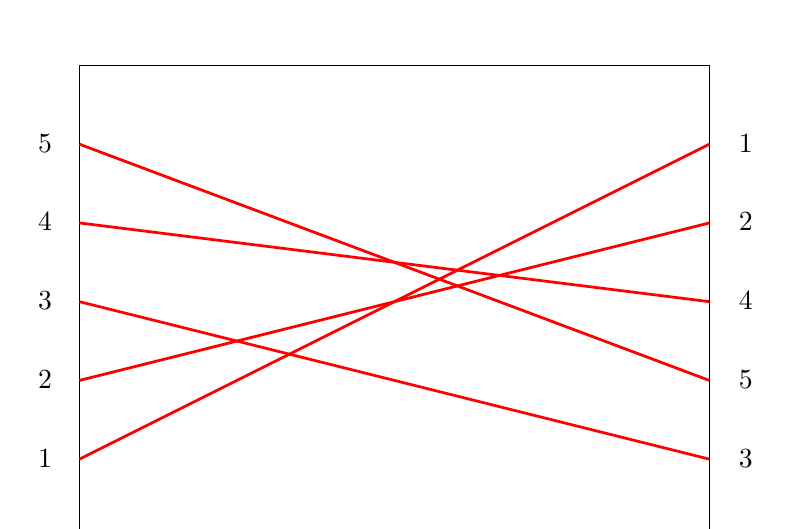
\begin{tikzpicture}
\draw[black, ultra thin] (-4,-3) rectangle (4,3);
\draw [line width=1pt,color=red] (-4,1)-- (4,0);
\draw [line width=1pt,color=red] (-4,-1)-- (4,1);
\draw [line width=1pt,color=red] (-4,0)-- (4,-2);
\draw [line width=1pt,color=red] (-4,2)-- (4,-1);
\draw [line width=1pt,color=red] (-4,-2)-- (4,2);
\draw (-4.65,2.25) node[anchor=north west] {5};
\draw (-4.65,1.25) node[anchor=north west] {4};
\draw (-4.65,0.25) node[anchor=north west] {3};
\draw (-4.65,-0.75) node[anchor=north west] {2};
\draw (-4.65,-1.75) node[anchor=north west] {1};
\draw (4.25,2.25) node[anchor=north west] {1};
\draw (4.25,1.25) node[anchor=north west] {2};
\draw (4.25,0.25) node[anchor=north west] {4};
\draw (4.25,-0.75) node[anchor=north west] {5};
\draw (4.25,-1.75) node[anchor=north west] {3};

\end{tikzpicture}
\caption*{Each inversion in the permutation displayed at the right represents an intersection of two lines inside the interval.} 
\end{figure}

That way, we can use variants of inversion counting algorithms in the implementation of \IntersectionsAndRandomIntersection. This will be done using Algorithm \ref{intersection_and_random_intersection_algorithm}, which transforms the range in a permutation of lines and then uses Algorithm \ref{inversions_and_random_inversion_algorithm}, which counts the inversions in a permutation and returns one chosen uniformly at random. Algorithm \ref{inversions_and_random_inversion_algorithm} runs in $\bigo(|G_1| \log |G_1|)$ time, as it is an adaptation of the well-known MergeSort algorithm for counting inversions.

%fazer ordenacao indireta talvez soh explicar o q fazer em vez de fazer
\begin{algorithm}
\begin{algorithmic}[1]
\Require{a set $G$ of lines in general position and an interval $T$}
\Ensure{the number of $T$-intersections of lines from $G$
        and a~random $T$-intersection of two lines from $G$}
\State $(a,b) \gets T$
\State $\textsc{SortEval}(G,a)$ 
\hfill {\small \textcolor{gray}{$\rhd G[1] \prec_a \cdots \prec_a G[|G|]$ }}
\State $\pi \gets \textsc{IndSortEval}(G,b)$ 
\hfill {\small \textcolor{gray}{$\rhd G[\pi[1]] \prec_b \cdots \prec_b G[\pi[|G|]]$ }}
\State $(c,u,v) \gets \textsc{InversionsAndRandomInversion}(\pi, 1,|\pi|)$
\If{$c=0$}\ \Return $(c,\None,\None)$ \EndIf 
\State $\inter \gets \textsc{intersection}(G[u],G[v])$
\State \Return $(c, \inter)$
\end{algorithmic}
\caption{\IntersectionsAndRandomIntersection$(G,a,b)$}
\label{intersection_and_random_intersection_algorithm}
\end{algorithm}

\begin{algorithm}
\begin{algorithmic}[1]
\Require{a permutation $\pi$ and integers $i$ and $j$ with $1 \leq i \leq j \leq |\pi|$}
\Ensure{the number of inversions in $\pi[i \tdots j]$ and a random pair of integers inverted 
in~$\pi[i \tdots j]$, if one exists. As a side effect, the algorithm sorts $\pi[i \tdots j]$.}
\If{$i=j$} \Return $(0,\None, \None)$ \EndIf \vspace{-1mm}
\State $k \gets \ceil{\frac{i+j}{2}}$
\State $(c_1,u_1,v_1) \gets \InversionsAndRandomInversion(\pi,i,k)$ 
\State $(c_2,u_2,v_2) \gets \InversionsAndRandomInversion(\pi,k+1,j)$ 

\State $c_3 \gets 0$ \hfill {\small \textcolor{gray}{$\rhd$ inversions between the two now sorted halves of $\pi$}}
\State $t_1 \gets i$ 
\State $t_2 \gets k+1$
\For{$t \in [i,j]$} \hfill {\small \textcolor{gray}{$\rhd$ similar to the Merge subroutine of MergeSort}}
    \If{$(t_1 \leq k \ \And \ t_2 \leq j \ \And \ \pi[t_1] < \pi[t_2])\ \Or \ t_2 > j$}
        \State $\pi'[t] \gets \pi[t_1]$
        \State $t_1 \gets t_1 + 1$
    \Else
        \State $c_3 \gets c_3 + k - t_1 + 1$
        \If{$c_3 > 0$} 
           \State $r \gets \rand(0,c_3)$
           \If {$r < k - t_1 + 1$} $u_3, v_3 \gets \pi[t_2],\pi[t_1+r]$ \EndIf \vspace{-1mm}
        \EndIf
        \State $\pi'[t] \gets \pi[t_2]$
        \State $t_2 \gets t_2 + 1$
    \EndIf \vspace{-1mm}
\EndFor
\For{$t \in [i,j]$} $\pi[t] \gets \pi'[t]$ \EndFor \vspace{-1mm}
\State $c \gets c_1 + c_2 + c_3$
\If{$c = 0$} \Return $(0, \None, \None)$ \EndIf \vspace{-1mm}
\State $r \gets \rand(0, c)$
\If{$r < c_1$} \Return $(c, u_1, v_1)$ \EndIf \vspace{-1mm}
\If{$r < c_1 + c_2$} \Return $(c, u_2, v_2)$ \EndIf \vspace{-1mm}
\State \Return $(c, u_3, v_3)$
\end{algorithmic}
\caption{\InversionsAndRandomInversion$(\pi, i, j)$}
\label{inversions_and_random_inversion_algorithm}
\end{algorithm}

\newpage
\subsubsection{Checking the Odd Intersection Property}


To see if an interval has the odd intersection property in relation to $L_{p_1}(G_1)$ and $L_{p_2}(G_2)$, we only have to check whether $L_{p_1}(G_1)$ and $L_{p_2}(G_2)$ changed order in that interval (e.g. $L_{p_1}(G_1)$ was below $L_{p_2}(G_2)$ at the beggining of the interval but above it at the end of the interval: by continuity, they must have intersected an odd number of times), which is what we do in Algorithm \ref{odd_level_intersection_algorithm}.

\begin{algorithm}
\begin{algorithmic}[1]
\Require{sets $G_1$ and $G_2$ of lines in general position, integers $p_1$ and $p_2$ with 
  $1 \leq p_1 \leq |G_1|$ and $1 \leq p_2 \leq |G_2|$ and an interval $T$}
\Ensure{Returns $\true$ if $L_{p_1}(G_1)$ and $L_{p_2}(G_2)$ intersect an odd number of times in $[a,b]$ and $\false$ otherwise}
 \State $(a,b) \gets T$
\State $g_1 \gets \textsc{Quickselect}(G_1,0,|G_1|,p_1,a)$
\hfill {\small \textcolor{gray}{$\rhd$ $L_{p_1}(G_1)$ at $x = a$ is on line $g_1$}}
\State $g_2 \gets \textsc{Quickselect}(G_2,0,|G_2|,p_2,a)$
\hfill {\small \textcolor{gray}{$\rhd$ $L_{p_2}(G_2)$ at $x = a$ it on line $g_2$}}
\State $\mathit{order}_a \gets \Eval(g_1, a) < \Eval(g_2, a)$
\hfill {\small \textcolor{gray}{$\rhd$ \true\ iff $L_{p_1}(G_1)$ is below $L_{p_2}(G_2)$ at $x = a$}}

\State $g_1 \gets \textsc{Quickselect}(G_1,0,|G_1|,p_1,b)$
\hfill {\small \textcolor{gray}{$\rhd$ $L_{p_1}(G_1)$ at $x = b$ is on line $g_1$}}
\State $g_2 \gets \textsc{Quickselect}(G_2,0,|G_2|,p_2,b)$
\hfill {\small \textcolor{gray}{$\rhd$ $L_{p_2}(G_2)$ at $x = b$ is on line $g_1$}}
\State $\mathit{order}_b \gets \Eval(g_1, b) < \Eval(g_2, b)$
\hfill {\small \textcolor{gray}{$\rhd$ \true\ iff $L_{p_1}(G_1)$ is below $L_{p_2}(G_2)$ at $x = b$}}
\State \Return $\mathit{order}_a \neq \mathit{order}_b$
\end{algorithmic}
\caption{\textsc{OddLevelIntersection}$(G_1,G_2,p_1,p_2,T)$}
\label{odd_level_intersection_algorithm}
\end{algorithm}

We will determine what is the $p$-th line of a set of lines $G$ when it is sorted by increasing evaluation at a given $x$ using the $\bigo(|G|)$ function \textsc{Quickselect}$(G,i,j,p,x)$, where $i$ and $j$ define the subinterval of $G$ we are know our answer is in; initially, $i=1$ and $j=|G|$.

\begin{algorithm}
\begin{algorithmic}[1]
\Require{{a set $G$ of lines, indices $i$ and $j$ such that $1\leq i \leq j\leq |G|$, an index $p$ such that $1\leq p\leq i-j+1$ and a coordinate $x$}}
\Ensure{{the $p$-th line of $G$ when sorted by increasing evaluation at $x$}}

\State $r \gets \rand(i,j+1)$
\State $id \gets i$
\State $G[r] \leftrightarrow G[j]$
\For{$k \in (i,j)$}
    \If{$\Eval(G[k],x) < \Eval(G[j])$}
    \State $G[k] \leftrightarrow G[id]$
    \State $id\gets id+1$
    \EndIf
\EndFor
\State $G[j]  \leftrightarrow G[id]$
\If{$id - i +1 > p$} \hfill {\small \textcolor{gray}{$\rhd$ the answer is to the left}}
\State \Return \textsc{Quickselect}$(G, i,id-1,p,x)$
\EndIf
\If{$id - i +1 < p$} \hfill {\small \textcolor{gray}{$\rhd$ the answer is to the right}}
\State \Return \textsc{Quickselect}$(G,id+1,j,p-(id-i+1),x)$
\EndIf
\State \Return $G[id]$
\end{algorithmic}
\caption{\textsc{Quickselect}$(G,i,j,p,x)$}
\label{quickselect_algorithm}
\end{algorithm}

With that, \textsc{OddLevelIntersection} has a final complexity of $\bigo(|G_1|+|G_2|)$, which is important because we will be using it later in our linear implementation of the  \textsc{NewInterval} function.

\newpage
\subsection{Finding the Trapezoid}

Now we will present a linear-time implementation of \textsc{FindTrapezoid}$(G,p,T)$ as previously described. We currently have an interval $T$ that has the odd intersection property in relation to $L_{p_1}(G_1)$ and $L_{p_2}(G_2)$. 

According to [1], the left side of the $T$-trapezoid will be bounded by the $(p_1 - \epsilon |G_1|)$-th and the $(p_1 + \epsilon |G_1|)$-th lines of $G_1$ when these lines are sorted by evaluation at the left side of $T$. Analogously, the right side of the $T$-trapezoid will be bounded by the $(p_1 - \epsilon |G_1|)$-th and the $(p_1 + \epsilon |G_1|)$-th lines of $G_1$ when these lines are sorted by evaluation at the right side of $T$.

Using $\epsilon = \frac{1}{8}$, that is enough for less than half of the lines in $G_1$ to be inside the $T$-trapezoid and for the $T$-trapezoid to contain the entirety of $L_{p_1}(G_1)$ in $T$.

That means that we need to be able to determine what is the $p$-th line of a set of lines $G$ when it is sorted by increasing evaluation at a given $x$. That can be done in linear time using the \textsc{Quickselect}$(G,i,j,p,x)$ function described in Algorithm \ref{quickselect_algorithm}.

With that, our final algorithm to find the trapezoid is as shown below:

\newcommand{\offset}{\mathit{offset}}


\begin{algorithm}
\begin{algorithmic}[1]
\Require{{a set $G$ of lines in general position, an integer $p$ such that $1\leq p \leq |G|$ and an interval $T$}}
\Ensure{{a trapezoid $\tau$ that contains less than half of the lines in $G$ and that contains the entirety of $L_{p}(G)$}}
\State $(a,b)\gets T$
\State $\offset \gets \floor{\frac{|G|}{8}}$
\State $left_{up} \gets \Eval$(\textsc{Quickselect}($G, (1,|G|),p+\offset,a),a$) \hfill {\small \textcolor{gray}{$\rhd$ $L_{p+\offset}(G)$ at $a$}}
\State $left_{down}\gets \Eval$( \textsc{Quickselect}($G, (1,|G|),p-\offset,a), a$)  \hfill {\small \textcolor{gray}{$\rhd$ $L_{p-\offset}(G)$ at $a$}}
\State $right_{up} \gets \Eval$( \textsc{Quickselect}($G, (1,|G|),p+\offset,b),b$)  \hfill {\small \textcolor{gray}$\rhd$ {$L_{p+\offset}(G)$ at $b$}}
\State $right_{down} \gets \Eval$(\textsc{Quickselect}($G,(1,|G|),p-\offset,b$), $b$)  \hfill {\small \textcolor{gray}{$\rhd$ $L_{p-\offset}(G)$ at $b$}}

\State $\tau \gets (left_{up}, left_{down}, right_{up}, right_{down})$
\State \Return $\tau$
\end{algorithmic}
\caption{\textsc{FindTrapezoid}$(G,p,T)$}
\label{find_trapezoid}
\end{algorithm}

\newpage
\subsection{Discarding the lines}

Lastly, we need to discard all lines from $G_1$ that do not intersect $\tau$ and update $p_1$ accordingly. We will do this using the function \textsc{DiscardLines}($G$,$p$,$\tau$), that receives a set $G$ of lines in general position, an integer $p$ such that $1\leq p \leq |G|$ and a $T$-trapezoid $\tau$. The fuction modifies $G$ and $p$ by removing all lines in $G$ that do not intersect $\tau$ and decreasing $p$ for every lines strictly below $\tau$ that was removed.

This can be done by simply going through all lines in $G$ and checking if they intersect $\tau$. Aditionally, if any lines are strictly below $\tau$, $p$ must be decreased by one. We can do that in linear time, as shown in Algorithm \ref{discardlines}.

In this algorithm we use two subroutines: \textsc{Intersects}$(\tau,g)$, that returns $\true$ if the line $g$ intersects the trapezoid $\tau$ and \textsc{Above}$(\tau,g)$, that returns $\true$ if $\tau$ is strictly above $g$.

%eu nao mudei as coisas faladas por que eu nao acho que faz sentido remover elementos de um vetor enquanto eu itero por ele
\begin{algorithm}
\begin{algorithmic}[1]
\Require{{a set $G$ of lines, an index $p$ such that $1\leq p \leq |G|$ and a trapezoid $\tau$}}
\Ensure{{the algorithm modifies $G$ and $p$ by removing all lines in $G$ that do not intersect $\tau$ and decreasing $p$ for every lines strictly below $\tau$ that was remove}}
\State $G^* \gets \{\}$
\For{$g \in G$}
\If{\textsc{Intersects}$(\tau,g)$} $G^* += g$ \EndIf
\If{\textsc{Above}$(\tau,g)$} $p \gets p - 1$ \EndIf
\EndFor
\State $G \gets G^*$
\end{algorithmic}
\caption{\textsc{DiscardLines}($G$,$p$,$\tau$)}
\label{discardlines}
\end{algorithm}

\newpage
\subsection{Brute Force}

When we have a sufficiently small number of lines, we need to brute-force a $T$-intersection between $L_{p_1}(G_1)$ and $L_{p_2}(G_2)$. We will use here a variant of Algorithm \ref{dual_n3_algorithm} that also takes into account the levels we want the intersection of.

\begin{algorithm}
\begin{algorithmic}[1]
    \Require{a set $G$ of lines an index $p$ and a point $i$}
    \Ensure{\textsc{true} if $i$ is in the $p$-th level of $G$ and \textsc{false} otherwise}
    
    \State $below \gets 0$
    \For{each line $g$ in $G$}
        \If{$i.y < g.m \cdot i.x + g.b $} $below \gets below + 1$
        \EndIf
    \EndFor
    \State \Return $below + 1 = p$
    \end{algorithmic}
    \caption{\textsc{IsPthLevel}($G,p,i$)}
    \label{ispthlevel}
\end{algorithm}

\begin{algorithm}
\begin{algorithmic}[1]
\Require{two nonempty sets $G_1$ and $G_2$ of lines, indices $p_1$ and $p_2$ and an interval $T$}
\Ensure{a point $i$ that is a $T$-intersection between $L_{p_1}(G_1)$ and $L_{p_2}(G_2)$}

 \For{each line $g_1$ in $G_1$}
  \For{each line $g_2$ in $G_2$}
    \State $x \gets \frac{g_2.b - g_1.b}{g_1.m - g_2.m}$
    \State $y \gets g_1.m \cdot x +g_1.b $
    \State $i \gets (x,y)$  \hfill {\small \textcolor{gray}{$\rhd$ intersection of $g_1$ and $g_2$}}
    \If{$x \in T$ \And \textsc{IsPthLevel}($G_1,p_1,i$) \And \textsc{IsPthLevel}($G_2,p_2,i$)} \Return{$i$}
    \EndIf
  \EndFor
 \EndFor
\end{algorithmic}
\caption{\textsc{BruteForce}($G_1,G_2,p_1,p_2, T$)}
\label{bruteforce}
\end{algorithm}

\newpage
\section{Finding a new interval in linear time}\label{sec:linear}

We will now discuss a linear implementation of the function \textsc{NewInterval}$(G_1,G_2,p_1,p_2,T)$, that receives two sets of lines $G_1$ and $G_2$ in general position, two integers $p_1$ and $p_2$ such that $1 \leq p_i \leq |G_i|$ and an interval $T$ on the $x$-axis with the odd intersection property in relation to $L_{p_1}(G_1)$ and $L_{p_2}(G_2)$ and returns an interval $T'\subset T$ that contains no more than $\alpha \times {|G_1| \choose 2}$ intersections among the lines in $G_1$ and that also has the odd intersection property in relatin to $L_{p_1}(G_1)$ and $L_{p_2}(G_2)$. This implementation was described in \cite{LoMS1994}.

The main idea of the algorithm is to split the whole $x$-axis in a constant number of intervals $T_1, \dots, T_C$, each of them containing no more than a fraction $\alpha \times {|G_1|\choose 2}$ of the intersections among the lines in $G_1$.

Then for every $i \in [C]$ we check if the interval $T \cap T_i$ (if it is non-empty) has the odd intersection property. Since $T_1, \dots, T_C$ spans the whole $x$-axis, one of them must have such property and be a feasible solution.

Firstly we will assume we have a function \textsc{FindAproximateIntersections}$(G,k,\delta)$ that receives a set $G$ of lines in general position, an integer $k$ such that $1 \leq k \leq {|G|\choose 2}$ and a real number $\delta$ such that $0 < \delta < 1$ and returns an $x$-coordinate $a$ such that the number $s$ of intersections of lines in $G$ lying to the left of the vertical line $x=a$ satisfies $|k-s|\leq \delta {G \choose 2}$. In other words, \textsc{FindAproximateIntersections}$(G,k,\delta)$ find an intersection that deviates from the $k$-th one by at most $ \delta {G \choose 2}$ intersections .The implementation of this function that we will use is described in \cite{epsnets} and runs in $\bigo(|G| \log \frac{1}{\delta}^3)$.

Take $N = {|G_1| \choose 2}$. Let $t_1<\dots < t_{N}$ be the $x$-coordinates of all the intersections of lines in $G_1$.
(Consider $t_j = -\infty$ if $j \leq 0$ and $t_j = \infty$ if $j>N$.) Given a certain integer $k$ with $1 \leq k \leq N$ and $\delta$, \textsc{FindAproximateIntersections} can be used to find the $x$-coordinate of an intersection between lines in $G_1$ in the interval $[t_{\ceil{k-\delta{N}}},t_{\ceil{k+\delta{N}}})$. We want to use that to find intervals $T_1, \dots, T_C$ as they were described above.

For $1\leq i \leq \floor{\frac{2}{\alpha}}$, let $u_i$ denote the output of \textsc{FindAproximateIntersections} with $G=G_1$, $k=\ceil{i \frac{\alpha}{2} N}$ and $\delta=\frac{\alpha}{4}$.  From the description of the algorithm, we know $u_i$ lies in the interval $[t_{\ceil{(i-\frac{1}{2}) \frac{\alpha}{2}{N}}},t_{\ceil{(i+\frac{1}{2}) \frac{\alpha}{2}{N}}})$ and we define $T_i$, for $1\leq i \leq \floor{\frac{2}{\alpha}} +1$,  as the interval $[u_{i-1},u_i)$, with $u_0 = -\infty$ and $u_{\floor{\frac{2}{\alpha}}+1}=\infty$. We can see that for every $i$, the largest possible number of intersections contained in
~$T_i$ is
\begin{align*}
\left\lceil\left(i+\frac{1}{2}\right) \frac{\alpha}{2}{N}\right\rceil-\left\lceil\left((i-1)-\frac{1}{2}\right)\frac{\alpha}{2}{N}\right\rceil -1 & \leq 
\left(i+\frac{1}{2}\right) \frac{\alpha}{2}{N}+1-\left((i-1)-\frac{1}{2}\right)\frac{\alpha}{2}{N} - 1\\
 & =\frac{\alpha}{2}{N} \left(\left(i+\frac{1}{2}\right)-\left((i-1)-\frac{1}{2}\right)\right) +1 -1\\
 & = \frac{\alpha}{2}{N} \left(i+\frac{1}{2}-(i-1)+\frac{1}{2})\right)  \\
 & = \frac{\alpha}{2}{N} \left(2\right) \\
 & = \alpha{N}.
\end{align*}

%definir um ultimo intervalo

Additionally, we only need to find $u_i$ for $1\leq i \leq \floor{\frac{2}{\alpha}}$ to guarantee that all intersections among the lines in $G_1$ will be contained in some interval $T_i$. Since $\alpha$ is a constant, we will be making at most  $\floor{\frac{2}{\alpha}}$ calls of the $\bigo(|G_1| \log \frac{1}{\delta}^3)\equiv \bigo(|G_1| \log \frac{1}{\alpha/4}^3)\equiv \bigo(|G_1|)$ function \textsc{FindAproximateIntersections} and $\floor{\frac{2}{\alpha}}$ calls of \textsc{OddLevelIntersection}, which runs in $\bigo(|G_1|+|G_2|)$, leading to a final complexity of $\bigo(|G_1|+|G_2|)$.

Below is the pseudocode for the algorithm, that uses both \textsc{FindAproximateIntersections} as described above and  \textsc{OddLevelIntersection} as described in Algorithm \ref{odd_level_intersection_algorithm}. It also uses as an auxiliary function \textsc{IntervalIntersection}$(T,T')$ that takes two intervals $T$ and $T'$ and returns their intersection.

%arrumar pra u0 e uzao
\begin{algorithm}
\begin{algorithmic}[1]
\Require{{sets $G_1$ and $G_2$ of lines in general position, two integers $p_1$ and $p_2$ such that $1 \leq p_i \leq |G_i|$ and an interval~$T$ in which $L_{p_1}(G_1)$ and $L_{p_2}(G_2)$ intersect an odd number of times}}
\Ensure{{an interval $T'\subset T$ that contains no more than $\alpha\times {|G_1|\choose 2}$ intersections among the lines in $G_1$ and in which $L_{p_1}(G_1)$ and $L_{p_2}(G_2)$ intersect an odd number of times}}
\State $\alpha \gets \frac{1}{32}$
\State $\delta \gets \frac{\alpha}{4}$
\State $u_0 \gets -\infty$
\For{$i \in [1,\left\lfloor \frac{2}{\alpha}\right\rfloor]$}
    \State $u_i \gets \textsc{FindAproximateIntersections}(G_1,\ceil{i \frac{\alpha}{2} N},\delta)$
    \State $T' \gets [u_{i-1},u_i)$
    \State $TT' \gets \textsc{IntervalIntersection}(T,T')$
    \If{$TT'\neq \emptyset$ \And \textsc{OddLevelIntersection}$(G_1,G_2,p_1,p_2,TT')$}
        \State \Return $TT'$
    \EndIf
\EndFor
\State $T'\gets [u_{\left\lfloor \frac{2}{\alpha}\right\rfloor},+\infty)$   
\State $TT' \gets \textsc{IntervalIntersection}(T,T')$
\State \Return $TT'$
\end{algorithmic}
\caption{\textsc{NewInterval}$(G_1,G_2,p_1,p_2,T)$}
\label{new_interval_linear_algorithm}
\end{algorithm}

\newpage

\subsection{Sorting Networks and $\epsilon$-Sorting Networks}

A sorting network is a device that can be used to efficiently sort an array when multiple distinct pairs of elements can be compared at the same time. What follows is one of the possible formalizations of this structure, described in \cite{epsnets}.
\begin{displayquote}

A \textit{parallel step} $P$ of width $n$ is a set $P=\{(p_1,q_1),\dots,(p_s,q_s)\}$ of ordered pairs, such that $p_1,q_1,p_2,q_2,\dots,p_s,q_s$ are distinct members of $[n]$(thus $s\leq n/2$). The ordered pair $(p_i,q_i)$ is called a \textit{comparator}. A network $H$ of width $n$ and depth $D$ is the ordered $D$-tuple $H=(P_1,P_2,\dots,P_D)$ where the $P_i$ are parallel steps of width $n$.

The computation of a network $H = (P_1, P_2,\dots, P_D)$ on an input vector
$(i_1,\dots, i_n)$ proceeds as follows: In the first step, $i_p$ is compared with $i_q$ for every
$(p, q) \in P_1$, and whenever $i_p > i_q$, these entries in the input vector are exchanged.
The input vector modified in this way is then processed by the second parallel step,
etc. 

The computation of the network obviously depends only on the permutation $\pi$,
which orders the input vector (i.e., such that $i_{\pi(1)}<i_{\pi(2)}<\dots<i_{\pi(n)}$). Let $H(\pi)$
denote the permutation performed on the input vector by the network when the
input vector is ordered by $\pi$. Thus, $H$ is a sorting network in the usual sense iff
$H(\pi) = \pi$ for every $\pi$. 

\end{displayquote}

We call a network $H$ an $\epsilon$-sorting network if for every permutation $\pi$ of size $n$, the number of inversions of that permutation after the computation of $H$ on $\pi$ ($H(\pi)\circ \pi^{-1}$) if less or equal to $\epsilon {n \choose 2}$. 

Aditionally, a network $H$ is an $t$-tolerant $\epsilon$-sorting network if any network $H'$ generated by deleting at most $t$ comparators from $H$ is an $\epsilon$-sorting network.

We will be further investigating properties of a specific sorting network described in \cite{AKS}, which we will call the AKS Sorting Network. It has depth of $\bigo(\log n)$ and can be used to prove the existence of sorting networks with certain properties, such as:

\begin{corollary}
There exists a constant $C$ such that, for $n \gg 1$ and $0 < v < 1$, we can
construct a $t$-tolerant $\epsilon$-sorting network $H = H(n, v)$ of width $n$ and of depth
$\bigo(\log v)$, where $t = \Omega(v^Cn)$. 
\end{corollary}

That is enough to describe the algorithm for \textsc{FindAproximateIntersections}.

\subsection{Approximately finding the $k$-th intersection}

We want to find a $\bigo(|G|\frac{1}{\delta}^3)$ algorithm for the function \textsc{FindAproximateIntersections}$(G,k,\delta)$ that receives a set $G$ of lines in general position, an integer $k$ such that $1 \leq k \leq {|G|\choose 2}$ and a real number $\delta$ such that $0 < \delta < 1$ and returns an $x$-coordinate $a$ such that the number $s$ of intersections of lines in $G$ lying to the left of the vertical line $x=a$ satisfies $|k-s|\leq \delta {G \choose 2}$.

Firstly we will describe a slower algorithm to find the $k$-th intersection among the lines in $G$, then we will apply the modifications needed for it to be more efficient. By making the algorithm more efficient, we will be performing some approximations, thus leading to the need of the parameter $\delta$.

The slower algorithm follows. Firstly, consider a sorting network $H$ and the $x$-coordinates of all the intersections among the lines in $G$ sorted by $x$-coordinate, which we will call $t_1, t_2, \dots, t_{|G| \choose 2}$. We are searching for $t_k$.

Now take the permutation that is formed when we sort the intercepts of lines in $G$ with the vertical line $x=t_k$. 


\newpage
\section{Our proposed algorithm}

\begin{algorithm}
\begin{algorithmic}[1]
\Require{{sets $G_1$ and $G_2$ of lines in general position, two integers $p_1$ and $p_2$ such that $1 \leq p_i \leq |G_i|$ and an interval~$T$ that has the odd intersection property in relation to $L_{p_1}(G_1)$ and $L_{p_2}(G_2)$}}
\Ensure{{an interval $T'\subset T$ such that the number of $T'$-intersections among the lines in $G_1$ is no more than $\alpha \times {|G_1| \choose 2}$ and that has the odd intersection property in relation to $L_{p_1}(G_1)$ and $L_{p_2}(G_2)$}}
\State $\alpha \gets \frac{1}{32}$
\State $divided \gets \true$
\While{$divided$}
\State $divided \gets \false$
\For{$ i \in [1,|G_1|]$}
\State $intersection \gets$ \textsc{RandomIntersection}($G_1$)
\If{$intersection \in T$}
\State $divided \gets \true$
\State $p \gets intersection.x$
\State $(a,b)\gets T$
\State $T_1 \gets (a,p.x)$
\State $T_2 \gets (p.x, b)$
\If{\textsc{OddLevelIntersection}($G_1$,$G_2$,$p_1$,$p_2$,$T_1$)}$\ T\gets T_1$
\Else $\ T\gets T_2$
\EndIf
\State break
\EndIf
\EndFor
\EndWhile
\State \Return $T$

\end{algorithmic}
\caption{\textsc{NewInterval}$(G_1,G_2,p_1,p_2,T)$}
\label{new_interval_algorithm}
\end{algorithm}

\bibliographystyle{plain}
\bibliography{references}

\end{document}